\documentclass{ctexart}
\usepackage{geometry}
\usepackage{graphicx}
\usepackage{hyperref}
\usepackage{paralist}
\usepackage{tikz}
\usepackage{amsmath}
\usepackage{xcolor}
\usepackage{multirow}
\usepackage{attachfile2}
\usepackage{pdfpages}
\usepackage{booktabs}
\usepackage[normalem]{ulem}
\usepackage{longtable}
\usepackage{float}
\usepackage[citestyle=verbose]{biblatex}
\usepackage{minted}
\attachfilesetup{color=red}

\addbibresource[location=local]{ref.bib}

\newminted{bash}{breakanywhere,breaklines,linenos,frame=single}

\title{数据结构课程设计 \\ 报告}
\author{队长:唐梓楠\ 2022211404 \\ 成员:马伟昊\ 2022211401 \\\phantom{成员:}张\quad 付\ 2022211396}
\date{\today}

\hypersetup{colorlinks=true,linkcolor=black,filecolor=magenta,urlcolor=cyan}

\begin{document}

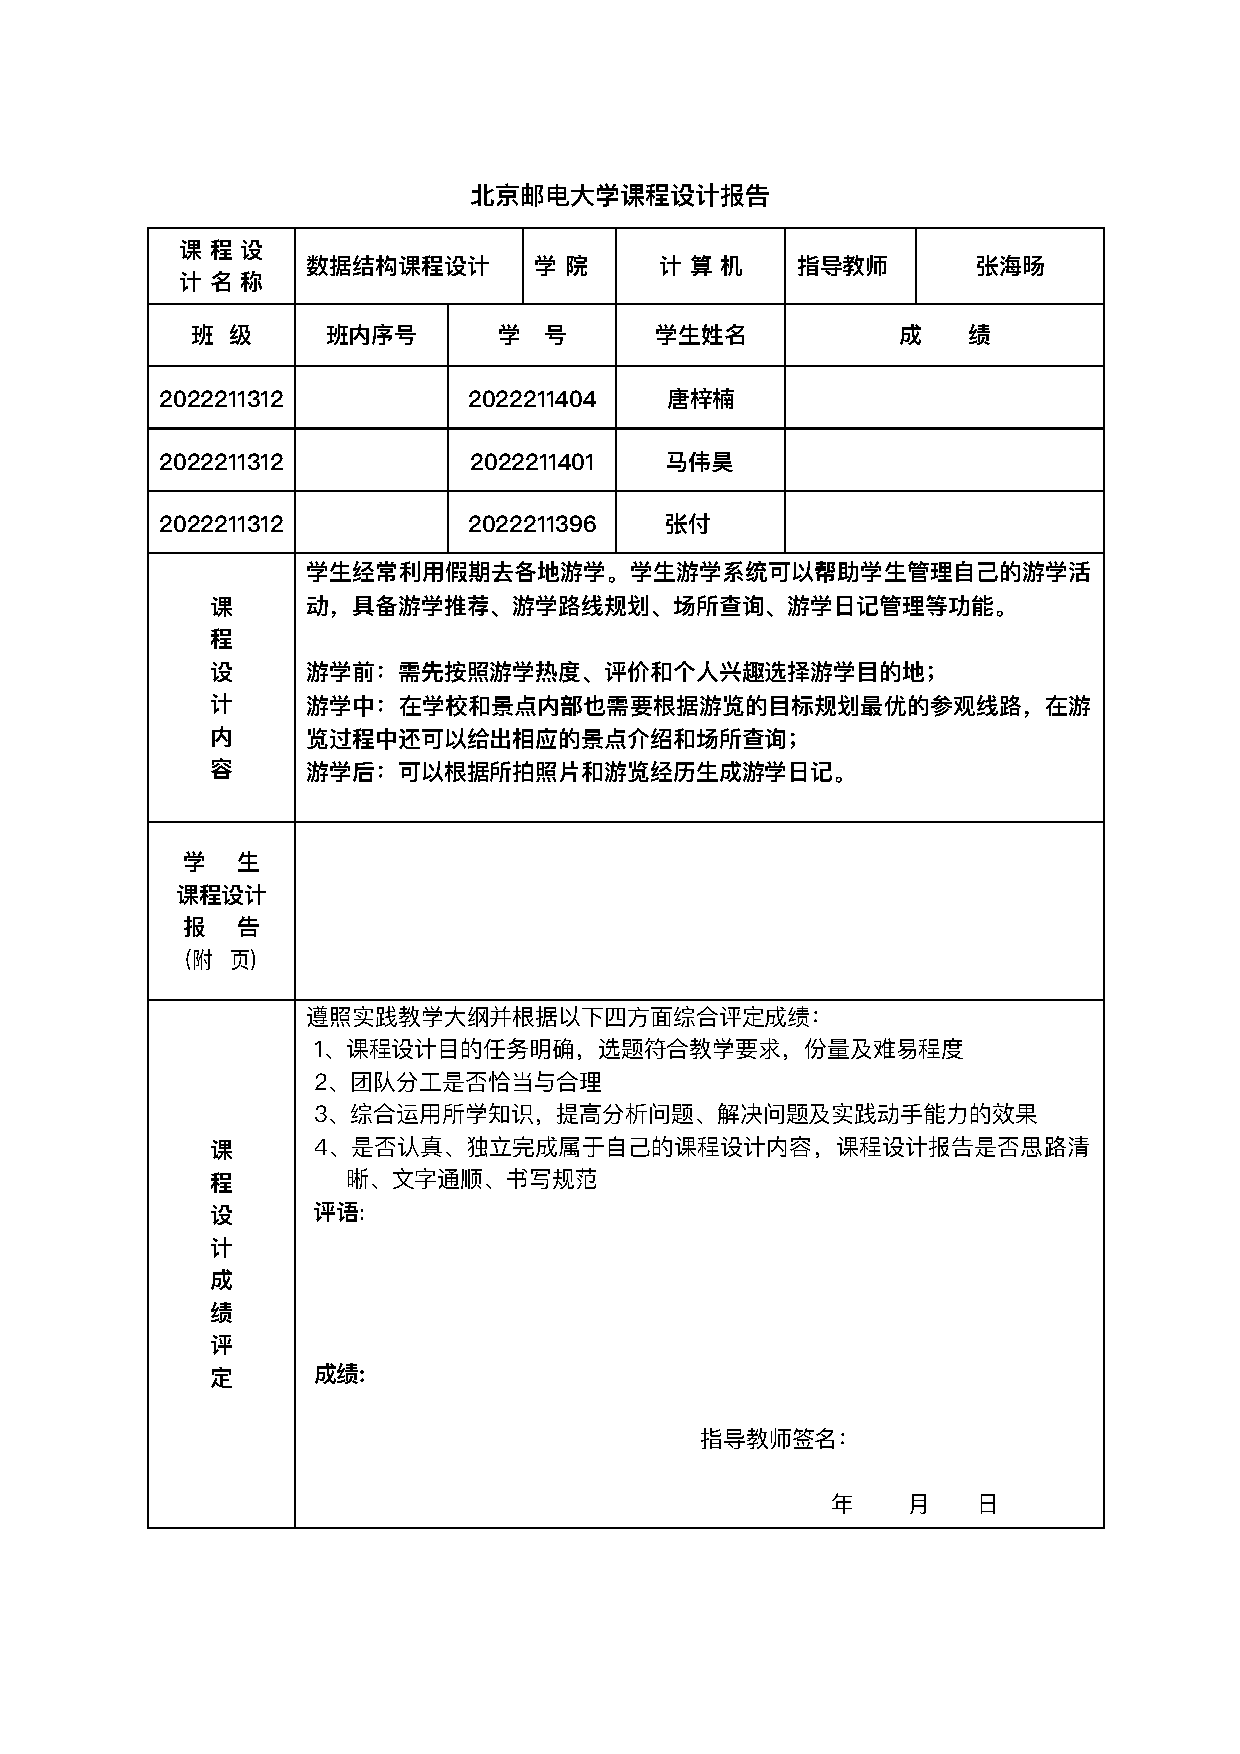
\includepdf[pages=-]{cover.pdf}

\tableofcontents

\newpage

\maketitle

\section{系统架构}

\subsection{技术栈}

\begin{compactdesc}
    \item[前端 JavaScript 框架:] Vue.js 3.4.0
    \item[前端 UI 组件框架:] Vuetify 3.5.0
    \item[其他主要前端组件:] wangEditor, 高德地图 JS API 2.0/ Web API
    \item[后端编程语言:] Python 3.12.3
    \item[后端 Web 应用框架:] Flask 3.0.3
    \item[数据库:] MySQL 8.3.0
\end{compactdesc}

\subsection{分工及学习路线图}

\subsubsection{唐梓楠}

全栈开发,同时负责前后端搭建,奠定项目基本框架以及过程开发,数据库搭建等工作,还负责大体文书工作。

\subsubsection{张付}
负责后端辅助开发以及算法:

\begin{itemize}
    \item 完成 Python 学习, \href{https://cs50.harvard.edu/python/2022/}{CS50P}, 看 Notes 即可;
    \item 在 windows 上配置好个人 git, 可自行搜索, 看 \textit{Pro Git} 等, 试着上传一份 hello world 代码到 github 仓库;
    \item 看 \href{https://tutorial.helloflask.com}{Flask 入门教程};
    \item 看 \href{https://dormousehole.readthedocs.io/en/latest/quickstart.html#}{Flask 官方文档};
    \item 如果遇到需要前端知识, 参照下文查漏补缺;
    \item 研究 Flask 和 Vue 如何配合。
\end{itemize}

\subsubsection{马伟昊}
负责前端辅助开发以及算法:

\begin{itemize}
    \item 完成 Python 学习, \href{https://cs50.harvard.edu/python/2022/}{CS50P}, 看 Notes 即可;
    \item 在 windows 上配置好个人 git, 可自行搜索, 看 \textit{Pro Git} 等, 试着上传一份 hello world 代码到 github 仓库;
    \item 看 \href{https://developer.mozilla.org/zh-CN/docs/Learn/Getting_started_with_the_web}{mdn web docs} 的 Web 入门, HTML, CSS, JavaScript, 工具与测试/Vue 部分;
    \item 看 \href{https://cn.vuejs.org/guide/introduction.html}{Vue 官方文档};
    \item 如果遇到需要前端知识, 参照上文查漏补缺;
    \item 研究 Flask 和 Vue 如何配合。
\end{itemize}

\subsection{文件结构}

\begin{bashcode}
    student-travel-system
    ├── README
    ├── backend
    │   ├── __init__.py
    │   ├── algorithm
    │   │   ├── B+tree.py
    │   │   ├── Leftmost Prefix Matching.py
    │   │   ├── a_star.py
    │   │   ├── greedy_tsp.py
    │   │   ├── merge_sort.py
    │   │   └── zlib and base64.py
    │   ├── animate_diff_lightning.py
    │   ├── app.py
    │   ├── config.py
    │   ├── mobius.py
    │   └── models.py
    ├── frontend
    │   ├── README.md
    │   ├── index.html
    │   ├── jsconfig.json
    │   ├── package.json
    │   ├── public
    │   │   └── favicon.ico
    │   ├── src
    │   │   ├── App.vue
    │   │   ├── assets
    │   │   │   ├── logo.png
    │   │   │   └── logo.svg
    │   │   ├── components
    │   │   │   ├── Detail.vue
    │   │   │   ├── Home.vue
    │   │   │   ├── LoginRegister.vue
    │   │   │   ├── README.md
    │   │   │   └── Travel.vue
    │   │   ├── main.js
    │   │   ├── plugins
    │   │   │   ├── README.md
    │   │   │   ├── index.js
    │   │   │   └── vuetify.js
    │   │   └── router.js
    │   ├── vite.config.mjs
    │   └── yarn.lock
    └── pyrightconfig.json
\end{bashcode}

\section{快速上手}

需要安装 \href{https://git-scm.com/}{Git}, \href{https://nodejs.org/}{Node.js}, \href{https://www.python.org/}{Python}, \href{https://www.mysql.com/}{MySQL} 等软件。

\begin{enumerate}
    \item 克隆项目到本地 \begin{bashcode}
              git clone https://github.com/Word2VecT/student-travel-system.git
              cd ./student-travel-system
          \end{bashcode}
    \item 安装前端依赖 \begin{bashcode}
              cd ./frontend
              yarn install
          \end{bashcode}
    \item 运行开发服务器 \begin{bashcode}
              yarn dev
          \end{bashcode}
    \item 进入后端目录 \begin{bashcode}
              cd ../backend
          \end{bashcode}
    \item 创建虚拟环境并激活 (\verb|venv|, \verb|virtualenv|, \verb|virtualenvwrapper|, \verb|pipenv| 等均可)

          以 \verb|virtualenvwrapper| 为例 \begin{bashcode}
              pip install virtualenv
              pip install virtualenvwrapper
              mkvirtualenv travel
              workon travel
          \end{bashcode}
    \item 安装后端依赖 \begin{bashcode}
              pip install -r requirements.txt
          \end{bashcode}
    \item 设置数据库, 确保你的 MySQL 服务正在运行,程序使用数据库用户名为 root,密码为空, 数据库名为 \verb|travel|, 也可以自行修改 \verb|./backend/config.py| 文件配置为本地
    \item 使用命令导入数据库 \begin{bashcode}
              mysql -u root -p < ./database/travel_2024-06-15.sql
          \end{bashcode}
    \item 运行 Flask 服务器 \begin{bashcode}
              flask run
          \end{bashcode}
    \item Enjoy!
\end{enumerate}

\section{完成功能}

\subsection{游学推荐}

\begin{itemize}
    \item 可以根据自己的喜好选择不同的景点和学校作为游学目的地;
    \item 系统会向学生推荐游学景点和学校,可以按照游学热度、评价和个人兴趣进行推荐;
    \item 可以根据景点级别 (如 5A 级景区),所在地区 (如海淀区) 进行筛选;
    \item 可以输入景点和学校的名称、关键字进行查询, 查询结果有多项时,可以对查询结果按照热度和评价进行排序。
\end{itemize}

\subsection{场所查询}

\begin{itemize}
    \item 在景区或者学校内部时,会找出所在位置附近一定范围内的超市、卫生间等服务设施,并根据距离进行排序;
    \item 可以通过输入类别对结果进行过滤;
    \item 可以由用户输入名称查找某个地点附近的服务设施,并根据距离进行排序。
\end{itemize}

\subsection{游学日记管理}

\begin{itemize}
    \item 可以撰写游学日记,通过文字的方式记录游学内容;
    \item 可以对所有学生的游学日记进行统一的管理;
    \item 可以根据浏览和查询所有学生的游学日记,游学日记的浏览量即为该日记的热度,每位同学浏览完可以对游学日记进行评分;
    \item 在浏览所有游学日记时,可以按照日记热度、评价进行推荐,推荐算法基础要求为排序算法,可以根据热度和评分进行排序;
    \item 可以输入游学目的地,对目的地相关的游学日记根据热度和评分进行排序;
    \item 可以输入游学日记的名称进行精确查询;
    \item 可以按日记内容进行全文检索;
    \item 可以对游学日记进行压缩存储。
\end{itemize}

\subsection{游学路线规划}

\begin{itemize}
    \item 当进入景区或者学校后,学生可以选择目标景点或者场所,系统会为学生规划从当前位置出发到达景点或者场所的最优游学线路;
    \item 进入景区或者学校后,学生可以输入多个目标景点或者场所信息,系统会为学生规划从当前位置出发,参观多个景点或者场所的最优游学线路;
    \item 线路规划可以按照最短距离策略或者最短时间策略进行规划;
    \item 可以选择步行、骑行两种出行方式进行线路规划。
\end{itemize}

\subsection{选做功能}

\begin{itemize}
    \item 设计导航功能的图形界面,包括地图展示和输出路径展示;
    \item 支持任意大型商场或知名建筑的室内导航;
    \item 按交通工具的最短时间策略;
    \item 美食推荐,在选中游览景点和学校后,可以按照距离进行排序,推荐附近的美食店;
    \item 采用推荐算法进行景点的推荐;
    \item 使用 AIGC 算法根据游学日记进行游学图片或动画生成。
\end{itemize}

\section{算法分析}

\begin{table}[htbp]
    \centering
    \caption{功能与算法对应表}
    \label{tab:my-table}
    \begin{tabular}{@{}cc@{}}
        \toprule
        \textbf{功能} & \textbf{使用算法}     \\ \midrule
        查找          & Hash 查找,B-tree 查找 \\
        排序          & B-tree 索引排序       \\
        最短路径        & A* ,贪心            \\
        文本搜索        & 倒排索引              \\
        文本压缩        & zlib,Base64       \\
        相似推荐        & TF-IDF,余弦相似度算法    \\
        AIGC        & Diffusion Model   \\
        \bottomrule
    \end{tabular}
\end{table}

\subsection{B-tree 查找}

\subsubsection{选用理由}

B-tree(平衡树)是常用的索引结构之一,适用于范围查找和顺序查找。

B-tree 索引是一种自平衡的树数据结构,能够保持数据有序,并提供高效的插入、删除和查找操作。

在 B-tree 中,每个节点可以包含多个键和指向子节点的指针。树的高度保持较低,从而确保操作的时间复杂度为 $O(\log n)$。

\subsubsection{应用场景}

B-tree 索引广泛应用于对表中数据进行快速查找。对景点的名称等字段进行查找时,使用 B-tree 索引。

\subsubsection{优点}

\begin{itemize}
    \item \textbf{高效查找}:B-tree 索引能够快速定位需要的数据,查找操作的时间复杂度为 $O(\log n)$;
    \item \textbf{支持范围查询}: B-tree 索引适用于范围查找,例如查找距离内的景点;
    \item \textbf{自动平衡}: B-tree 索引自动保持平衡,确保操作效率的一致性。
\end{itemize}

\subsubsection{缺点}

\begin{itemize}
    \item \textbf{维护成本}:维护 B-tree 索引需要额外的计算资源,特别是在插入和删除操作较多的情况下;
    \item \textbf{存储开销}:B-tree 索引需要额外的存储空间来存储索引结构。
\end{itemize}

\subsection{Hash 查找}

\subsubsection{选用理由}

Hash 索引基于哈希表数据结构,适用于精确查找操作。哈希表使用哈希函数将键映射到对应的存储位置,从而实现快速查找。
在 Hash 索引中,哈希函数计算出的哈希值用于定位数据存储的位置,这使得查找操作非常高效。

\subsubsection{应用场景}

Hash 索引适用于对唯一性或等值查找的场景。例如,在你的项目中,对用户的用户名进行查找时,可以使用 Hash 索引。

\subsubsection{优点}

\begin{itemize}
    \item \textbf{快速查找}:Hash 索引能够在常数时间内($O(1)$)完成查找操作,速度非常快。
    \item \textbf{简单高效}:Hash 索引的结构和查找算法相对简单,效率高。
\end{itemize}

\subsubsection{缺点}

\begin{itemize}
    \item \textbf{不支持范围查询}:Hash 索引不适用于范围查找操作,只能进行精确匹配查找。
    \item \textbf{哈希冲突}:哈希冲突可能会影响查找效率,需要额外的处理来解决冲突。
    \item \textbf{存储开销}:Hash 索引需要额外的存储空间来存储哈希表。
\end{itemize}

通过使用 Hash 索引算法,可以实现对唯一性或等值查找的高效存储和查询,适用于需要快速查找的场景,如对用户的用户名进行查找。

通过使用 B-tree 索引和 Hash 索引,实现了对景点和游记信息的高效存储和查找。这些查找算法在性能和适应性上各有优势,能够满足不同场景下的查询需求。B-tree 索引适用于范围查找和排序操作,而 Hash 索引适用于精确查找操作。通过结合使用这些索引结构,MySQL 能够在保证查找效率的同时,提供灵活的查询能力。

\subsection{B-tree 索引排序}

\subsubsection{选用理由}

B-tree(平衡树)是常用的索引结构之一。它是一种自平衡的树数据结构,能够保持数据有序,并提供高效的插入、删除和查找操作。

在排序操作中,B-tree 索引可以有效地快速定位数据并按照特定的顺序进行排列。

\subsubsection{应用场景}

对景点的热度(popularity)、评分(rating)、价格(price)进行排序时, 使用 B-tree 索引来加速查询和排序操作。

\subsubsection{优点}

\begin{itemize}
    \item \textbf{快速检索}:B-tree 索引结构使得查找操作的时间复杂度为 $O (\log n)$,能够快速定位需要的数据;
    \item \textbf{高效排序}:使用 B-tree 索引进行排序时,无需额外的排序操作,直接按照索引顺序读取数据即可;
    \item \textbf{自动平衡}:B-tree 自动保持平衡,确保每次操作后的树高度尽量保持在最低,从而保证操作效率。
\end{itemize}

\subsubsection{缺点}

\begin{itemize}
    \item \textbf{维护成本}:维护 B-tree 索引需要额外的计算资源,特别是在插入和删除操作较多的情况下;
    \item \textbf{存储开销}:B-tree 索引需要额外的存储空间来存储索引结构。
\end{itemize}

通过使用 B-tree 索引算法,实现了对景点和游记信息的高效存储和查询,适用于有明确排序需求的字段,如热度、评分和价格。

\subsection{TF-IDF 和余弦相似度算法}

\subsubsection{选用理由}

TF-IDF(Term Frequency-Inverse Document Frequency)和余弦相似度是文本挖掘和信息检索中常用的算法。TF-IDF 算法用于衡量一个词在一个文档中的重要性,而余弦相似度用于衡量两个向量(在这里是文档的向量表示)之间的相似度。通过结合使用这两个算法,可以高效地计算文本(如旅游景点描述)之间的相似性。

在推荐系统中,使用 TF-IDF 和余弦相似度可以根据描述文本找到相似的景点,为用户提供相关性高的推荐。

\subsubsection{应用场景}

TF-IDF 和余弦相似度算法适用于需要计算文本相似度的场景。例如,在旅游景点推荐系统中,可以使用这些算法根据景点描述文本计算相似度,找到相似的景点进行推荐。

\subsubsection{优点}

\begin{itemize}
    \item \textbf{高效性}:TF-IDF 和余弦相似度算法计算效率较高,适合大规模文本数据处理。
    \item \textbf{易于实现}:这些算法实现简单,容易理解和使用。
    \item \textbf{解释性强}:TF-IDF 能够衡量词语在文档中的重要性,余弦相似度能够量化文档之间的相似性,具有良好的解释性。
\end{itemize}

\subsubsection{缺点}

\begin{itemize}
    \item \textbf{忽略词序信息}:这些算法只考虑词频和词语的重要性,忽略了文本中的词序和语义信息,可能无法捕捉到复杂的语义关系。
    \item \textbf{停用词处理}:需要手动处理停用词(如“the”,“is”等),否则可能影响结果。
    \item \textbf{维度高}:对于大型文档集合,TF-IDF 向量的维度可能非常高,计算和存储开销较大。
\end{itemize}

通过使用 TF-IDF 和余弦相似度算法,可以高效地计算景点描述之间的相似度,为用户提供基于文本内容的相似景点推荐。

\subsection{A* 算法}

\subsubsection{选用理由}

A* 算法是一种启发式搜索算法,通过结合 Dijkstra 算法的优点和启发式函数(通常为估算的距离,如直线距离)来优化搜索过程。A* 算法在路径搜索中既考虑当前路径的成本,又考虑从当前节点到目标节点的预估成本,从而加速了路径搜索过程。

A* 算法常用大规模地图的路径搜索,因为它能够在保证找到最优路径的同时,提高搜索效率。

\subsubsection{应用场景}

A* 算法适用于需要在大规模图中快速找到最优路径的场景。用户指定起点和终点后,可以使用 A* 算法计算最短路径,并且在路径搜索中优先探索更有希望的路径。

\subsubsection{优点}

\begin{itemize}
    \item \textbf{高效性}:通过启发式函数引导搜索方向,能够显著减少搜索空间,提高搜索效率。
    \item \textbf{准确性}:在启发式函数满足一致性条件时,A* 算法保证找到最优路径。
    \item \textbf{灵活性}:启发式函数可以根据具体应用进行调整,适应不同的路径搜索需求。
\end{itemize}

\subsubsection{缺点}

\begin{itemize}
    \item \textbf{启发式函数依赖性}:算法性能高度依赖于启发式函数的选择,若启发式函数不准确,可能会降低搜索效率。
    \item \textbf{计算复杂度}:尽管比 Dijkstra 算法更高效,但在最坏情况下,时间复杂度仍为 $O(E + V\log V)$,在超大规模图上仍可能表现不佳。
    \item \textbf{内存消耗}:与 Dijkstra 算法类似,A* 算法在处理大图时需要大量内存。
\end{itemize}

通过使用 A* 算法,导航软件能够在大规模地图中快速找到最优路径,并提供高效的导航指引,特别适用于需要快速响应的大规模路径搜索场景。

\subsection{贪心算法求解旅行商问题 (TSP)}

\subsubsection{选用理由}

使用近似算法求解旅行商问题 (TSP) 是一种在求解复杂性高、难以找到最优解的情况下的有效策略。基于贪心算法的近似求解通过不断选择当前权重最小的边来构建路径,从而找到一个近似最优的解决方案。

在实际应用中,近似算法能够在合理的时间内找到一个较优的路径,特别适用于节点较多的图。

\subsubsection{应用场景}

近似算法适用于解决旅行商问题 (TSP),尤其是在节点数量较多、需要快速找到一个可行解的场景。在本项目中,我们用于途经多点最短路径算法,从当前位置出发,参观完返回当前位置的情况。

\subsubsection{优点}

\begin{itemize}
    \item \textbf{计算效率高}:近似算法能够在多项式时间内完成计算,适合大规模图的求解。
    \item \textbf{实现简单}:基于贪心策略的算法相对简单易实现,不需要复杂的优化技巧。
    \item \textbf{结果可接受}:虽然不是最优解,但近似解在大多数情况下足够接近最优解,满足实际应用需求。
\end{itemize}

\subsubsection{缺点}

\begin{itemize}
    \item \textbf{不能保证最优解}:近似算法不能保证找到最优解,只能找到一个接近最优的解。
    \item \textbf{依赖初始选择}:算法结果可能受初始选择的影响,可能存在局部最优解。
    \item \textbf{结果质量不稳定}:对于某些特定图,近似解的质量可能较差,需要结合具体应用场景进行评估。
\end{itemize}

这种方法特别适用于需要快速响应、对结果精度要求相对较低的场景。

\subsection{构建和查询倒排索引}

\subsubsection{选用理由}

全文搜索通过构建和查询倒排索引来实现快速的文本搜索。

倒排索引是一种数据结构,记录了文档中每个单词的位置,便于快速查找包含特定单词的文档。

通过构建和查询倒排索引来实现快速的文本搜索。

\subsubsection{优点}

\begin{itemize}
    \item \textbf{高效性}: 使用倒排索引,能够快速查找和匹配大量文本数据。
    \item \textbf{准确性}: 计算匹配度,能够返回最相关的搜索结果。
    \item \textbf{灵活性}: 支持多种查询模式,满足不同的搜索需求。
\end{itemize}

\subsubsection{缺点}

\begin{itemize}
    \item \textbf{索引维护开销}: 构建和维护倒排索引需要额外的存储空间和计算资源;
    \item \textbf{更新延迟}: 插入、更新和删除操作可能导致索引失效,需要定期重建索引;
    \item \textbf{语言依赖性}: 分词和匹配算法依赖于自然语言处理技术,可能对不同语言的支持效果不一。
\end{itemize}

\subsection{zlib 算法}

\subsubsection{选用理由}

zlib 是一种广泛使用的数据压缩库,基于 DEFLATE 压缩算法。DEFLATE 是一种无损压缩算法,结合了 LZ77 和哈夫曼编码算法,能够在保证数据完整性的同时显著减少数据体积。

在数据传输和存储中,使用 zlib 压缩算法可以有效节省带宽和存储空间,提高传输效率。

\subsubsection{应用场景}

zlib 压缩算法适用于各种需要数据压缩的场景。使用该算法对游学日记进行压缩存储。

\subsubsection{优点}

\begin{itemize}
    \item \textbf{高效压缩}:结合 LZ77 和哈夫曼编码,zlib 能够在保证数据完整性的同时提供高效的压缩率。
    \item \textbf{广泛兼容}:zlib 库被广泛支持,几乎在所有操作系统和编程语言中都可以使用。
    \item \textbf{无损压缩}:保证原始数据的完整性,压缩和解压缩后数据完全一致。
\end{itemize}

\subsubsection{缺点}

\begin{itemize}
    \item \textbf{计算复杂度高}:压缩和解压缩过程需要一定的计算资源,对性能有一定影响。
    \item \textbf{压缩比受限}:对于某些类型的数据(如已经压缩的文件或随机数据),压缩比可能不理想。
\end{itemize}

通过使用 zlib 压缩算法,可以在保证数据完整性的同时,显著减少数据传输和存储的体积,提高整体效率。

\subsection{Base64 编码算法}

\subsubsection{选用理由}

Base64 是一种用于表示二进制数据的编码方案,使用 64 个字符(包括字母、数字、加号和斜杠)来表示二进制数据。

在需要传输或存储二进制数据的场景中,使用 Base64 编码可以确保数据不会因字符编码问题而丢失或损坏。

\subsubsection{应用场景}

Base64 编码适用于需要在文本中嵌入二进制数据的场景。

由于 zlib 压缩后的数据是二进制数据,无法直接在文本中传输,因此需要使用 Base64 编码将二进制数据转换为文本数据,以便在文本中传输和存储。

\subsubsection{优点}

\begin{itemize}
    \item \textbf{文本友好}:Base64 编码的数据可以安全地嵌入到文本中,不会因字符编码问题而丢失或损坏。
    \item \textbf{广泛兼容}:Base64 编码被广泛支持,几乎所有编程语言和平台都提供了对 Base64 编码和解码的支持。
    \item \textbf{简单易用}:编码和解码过程简单,易于实现和使用。
\end{itemize}

\subsubsection{缺点}

\begin{itemize}
    \item \textbf{数据膨胀}:Base64 编码后的数据比原始数据大约膨胀了 33\%,在某些场景下会增加传输和存储的开销。
    \item \textbf{安全性低}:Base64 只是编码方式,不提供加密功能,不能保护数据安全。
\end{itemize}

\subsection{Diffusion Model}

\subsubsection{选用理由}

Diffusion Model(扩散模型)是一种用于生成图像和其他数据的生成模型。它基于对数据的逐步去噪过程,通过逐步添加噪声到数据,并训练模型在每一步去除噪声,最终生成逼真的数据样本。Diffusion Model 被证明在生成图像方面具有高效性和高质量。

在生成任务中,使用 Diffusion Model 可以生成高质量的图像,特别适用于需要生成逼真和复杂结构的场景。

\subsubsection{应用场景}

Diffusion Model 适用于各种生成任务,例如图像生成、视频生成。特别是在图像生成领域,Diffusion Model 已经被广泛应用于生成高质量的图片。用于游学日记生成配图或视频。

\subsubsection{优点}

\begin{itemize}
\item \textbf{生成质量高}:通过逐步去噪的过程,Diffusion Model 能够生成高质量的图像,具有逼真的细节和复杂的结构。
\item \textbf{训练稳定}:相比其他生成模型,Diffusion Model 的训练过程更稳定,不容易出现模式崩溃(mode collapse)问题。
\item \textbf{灵活性强}:Diffusion Model 可以灵活地应用于各种数据类型,包括图像、音频和文本等。
\end {itemize}

\subsubsection {缺点}

\begin{itemize}
    \item \textbf{计算开销大}:生成过程需要多步去噪,每一步都需要计算,导致生成过程较慢,计算资源消耗大。
    \item \textbf{训练时间长}:模型训练需要大量的数据和长时间的训练过程,对计算资源要求高。
    \item \textbf{复杂度高}:实现和调试 Diffusion Model 的算法较为复杂,涉及较多的参数调整和模型优化。
\end{itemize}

通过使用 Diffusion Model,可以在图像生成任务中获得高质量的生成结果,适用于对游学日记生成逼真图像。

\section{系统测试结果}

\subsection{游学推荐测试}

\begin{table}[H]
    \centering
    \caption{游学推荐功能测试结果}
    \begin{tabular}{|c|c|c|c|}
        \hline
        \textbf{测试用例} & \textbf{测试步骤} & \textbf{预期结果} & \textbf{实际结果} \\ \hline
        景点推荐          & 选择喜欢的景点类型     & 推荐相关景点        & 推荐结果符合预期      \\ \hline
        学校推荐          & 选择喜欢的学校类型     & 推荐相关学校        & 推荐结果符合预期      \\ \hline
        热度筛选          & 根据热度筛选景点和学校   & 显示高热度景点和学校    & 结果符合预期        \\ \hline
        关键字查询         & 输入景点或学校名称     & 查询到相关结果       & 结果符合预期        \\ \hline
    \end{tabular}
\end{table}

\subsection{场所查询测试}

\begin{table}[H]
    \centering
    \caption{场所查询功能测试结果}
    \begin{tabular}{|c|c|c|c|}
        \hline
        \textbf{测试用例} & \textbf{测试步骤} & \textbf{预期结果} & \textbf{实际结果} \\ \hline
        超市查询          & 输入超市类别        & 显示附近超市        & 显示结果正确        \\ \hline
        卫生间查询         & 输入卫生间类别       & 显示附近卫生间       & 显示结果正确        \\ \hline
        名称查询          & 输入服务设施名称      & 显示相关设施        & 显示结果正确        \\ \hline
        距离排序          & 按距离排序结果       & 显示按距离排序的结果    & 结果符合预期        \\ \hline
    \end{tabular}
\end{table}

\subsection{游学日记管理测试}

\begin{table}[H]
    \centering
    \caption{游学日记管理功能测试结果}
    \begin{tabular}{|c|c|c|c|}
        \hline
        \textbf{测试用例} & \textbf{测试步骤} & \textbf{预期结果} & \textbf{实际结果} \\ \hline
        日记撰写          & 撰写新的游学日记      & 成功保存日记        & 保存成功          \\ \hline
        日记评分          & 对游学日记进行评分     & 成功记录评分        & 评分记录成功        \\ \hline
        热度排序          & 根据热度排序日记      & 按热度显示排序结果     & 排序结果正确        \\ \hline
        内容检索          & 输入关键字搜索日记     & 显示相关日记        & 搜索结果正确        \\ \hline
        日记压缩          & 对日记进行压缩存储     & 成功压缩并存储       & 压缩存储成功        \\ \hline
    \end{tabular}
\end{table}

\subsection{游学路线规划测试}

\begin{table}[H]
    \centering
    \caption{游学路线规划功能测试结果}
    \begin{tabular}{|c|c|c|c|}
        \hline
        \textbf{测试用例} & \textbf{测试步骤} & \textbf{预期结果} & \textbf{实际结果} \\ \hline
        单点规划          & 输入单个目标地点      & 规划最优路线        & 路线规划正确        \\ \hline
        多点规划          & 输入多个目标地点      & 规划最优路线        & 路线规划正确        \\ \hline
        路线选择          & 选择步行或骑行方式     & 规划对应的路线       & 路线规划正确        \\ \hline
        最短时间          & 选择最短时间策略      & 显示最短时间路线      & 路线规划正确        \\ \hline
        最短距离          & 选择最短距离策略      & 显示最短距离路线      & 路线规划正确        \\ \hline
    \end{tabular}
\end{table}

\subsection{选做功能测试}

\begin{table}[H]
    \centering
    \caption{选做功能测试结果}
    \begin{tabular}{|c|c|c|c|}
        \hline
        \textbf{测试用例} & \textbf{测试步骤}  & \textbf{预期结果} & \textbf{实际结果} \\ \hline
        室内导航          & 选择大型商场内导航      & 显示室内导航路线      & 导航路线正确        \\ \hline
        美食推荐          & 选择景点或学校后查看美食推荐 & 显示附近美食推荐      & 推荐结果正确        \\ \hline
        AIGC生成        & 根据游学日记生成图片或动画  & 生成高质量图片或动画    & 生成结果符合预期      \\ \hline
    \end{tabular}
\end{table}

\section{功能改进建议}

在实际应用中,我们的系统需要更好地满足用户的需求。以下是用户反馈对各个功能模块的改进建议,以提升用户体验和系统实用性。

\subsection{游学推荐功能}

\begin{itemize}
    \item \textbf{丰富推荐维度}:除了景点和学校的推荐,可以增加活动、课程、讲座等内容的推荐,满足用户多样化的需求。
    \item \textbf{用户反馈机制}:添加用户反馈功能,让用户可以对推荐结果进行评价和反馈,帮助优化推荐算法。
\end{itemize}

\subsection{场所查询功能}

\begin{itemize}
    \item \textbf{动态更新服务设施信息}:确保服务设施的信息及时更新,特别是在景区或学校内的临时设施和活动。
    \item \textbf{用户评分和评论}:增加用户评分和评论功能,让用户可以对超市、卫生间等设施进行评价,方便其他用户参考。
    \item \textbf{导航功能}:提供从当前位置到目标设施的导航功能,帮助用户更方便地找到所需设施。
\end{itemize}

\subsection{游学日记管理功能}

\begin{itemize}
    \item \textbf{社交互动}:增加社交互动功能,让用户可以对游学日记点赞、评论和分享,增强用户之间的互动。
    \item \textbf{智能推荐}:基于用户的兴趣和浏览历史,智能推荐相关的游学日记,提高日记的曝光率和阅读量。
\end{itemize}

\subsection{游学路线规划功能}

\begin{itemize}
    \item \textbf{实时路况信息}:集成实时路况信息,帮助用户避开拥堵路段,优化路线规划。
    \item \textbf{自定义路线规划}:允许用户根据自己的需求自定义路线,并在系统推荐的基础上进行调整。
    \item \textbf{语音导航}:提供语音导航功能,特别是在骑行和步行模式下,提升用户的使用体验。
\end{itemize}

\subsection{选做功能}

\begin{itemize}
    \item \textbf{增强图形界面}:设计更加直观和美观的图形界面,提升用户的视觉体验和操作便利性。
    \item \textbf{多语言支持}:考虑到不同用户的需求,增加对多种语言的支持,提升系统的国际化水平。
    \item \textbf{智能推荐算法}:引入更多先进的推荐算法,如协同过滤和深度学习模型,提高推荐结果的准确性和用户满意度。
    \item \textbf{AIGC算法优化}:不断优化 AIGC 算法,提升生成图片和动画的质量和多样性,满足用户个性化需求。
\end{itemize}

通过以上改进,我们的系统将能够更好地满足用户的实际需求,提升用户体验和系统实用性。在未来的开发中,我们将继续关注用户反馈,不断优化和完善系统功能。

\section{使用大模型辅助设计和开发}

在系统设计和开发过程中,利用大模型可以显著提升工作效率和产品质量。以下是我们小组在开发过程中的具体的使用方法:

\subsection{需求分析与功能设计}

\begin{itemize}
    \item \textbf{需求文档生成}:利用大模型自动生成和完善需求文档,确保所有功能和需求明确记录,减少沟通成本。
    \item \textbf{用户反馈分析}:通过大模型分析用户反馈,提取关键意见和建议,快速响应并调整设计方案。
    \item \textbf{市场调研}:使用大模型进行市场调研和竞品分析,获取最新的行业动态和趋势,辅助决策。
\end{itemize}

\subsection{代码开发与优化}

\begin{itemize}
    \item \textbf{代码生成与补全}:利用大模型自动生成和补全代码,提升开发效率,减少手动编码的错误和重复劳动。
    \item \textbf{算法优化}:使用大模型分析现有算法,提出优化建议,提升系统性能和效率。
    \item \textbf{代码重构与审查}:通过大模型进行代码重构和审查,发现潜在的代码问题和优化点,提高代码质量和可维护性。
\end{itemize}

\subsection{测试与调试}

\begin{itemize}
    \item \textbf{自动化测试用例生成}:利用大模型自动生成测试用例,覆盖更多测试场景,提升测试效率和覆盖率。
    \item \textbf{错误分析与修复}:通过大模型自动分析测试结果和错误日志,快速定位问题并提出修复建议。
    \item \textbf{用户行为模拟}:使用大模型模拟用户行为,进行压力测试和性能测试,确保系统在高负载下的稳定性。
\end{itemize}

\subsection{用户体验提升}

\begin{itemize}
    \item \textbf{自然语言处理}:利用大模型的自然语言处理能力,提升系统与用户交互的智能化水平,例如语音识别和自然语言查询。
    \item \textbf{个性化推荐}:通过大模型分析用户行为和偏好,提供个性化的推荐和内容推送,提升用户满意度。
    \item \textbf{多媒体内容生成}:使用大模型生成高质量的图片、视频和音频,丰富系统的多媒体内容表现形式。
\end{itemize}

\subsection{持续集成与部署}

\begin{itemize}
    \item \textbf{自动化部署脚本生成}:利用大模型自动生成和优化部署脚本,简化持续集成与部署流程,减少人为错误。
    \item \textbf{监控与预警}:通过大模型进行系统监控和预警,提前发现潜在问题,确保系统的高可用性和稳定性。
    \item \textbf{日志分析}:使用大模型自动分析系统日志,提取关键信息和异常情况,提升运维效率。
\end{itemize}

通过将大模型应用于系统设计和开发的各个环节,我们可以显著提升系统的智能化水平和用户体验,确保系统能够更好地满足用户的实际需求。

\section{运行效果展示}

\begin{figure}[htbp]
    \centering
    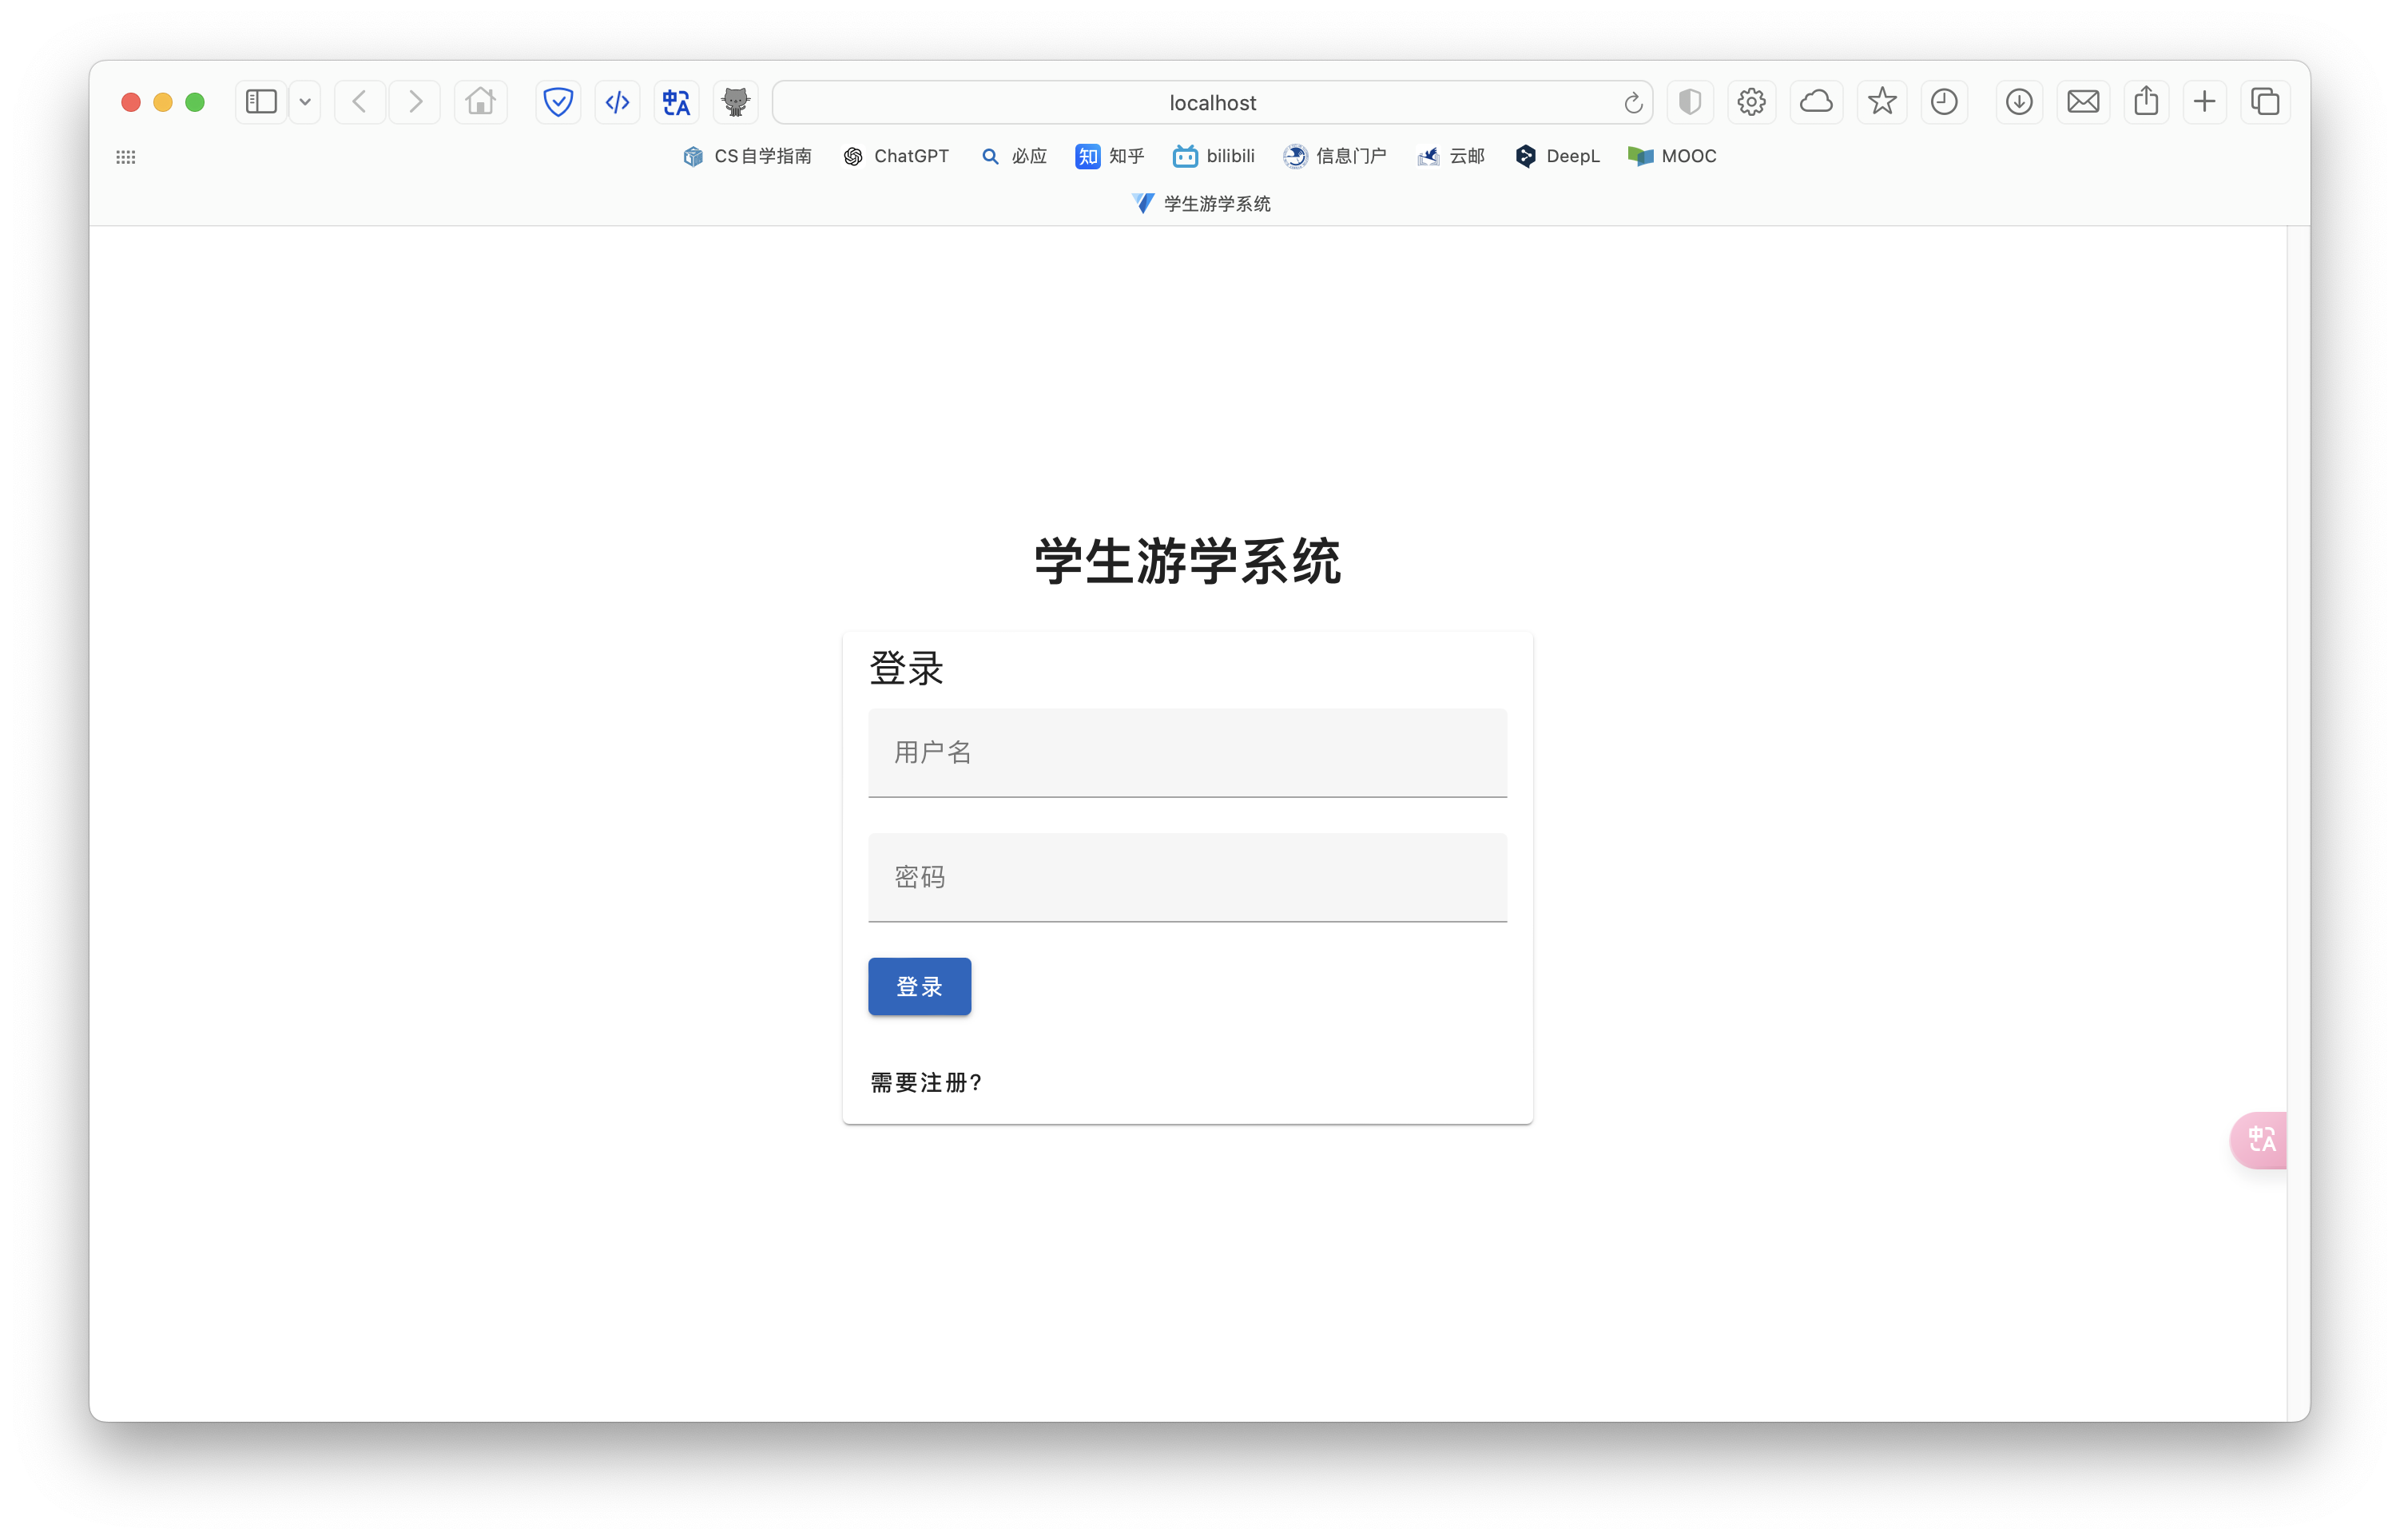
\includegraphics[width=0.85\textwidth]{figure/login.png}
    \caption{登录界面}
\end{figure}

\begin{figure}[htbp]
    \centering
    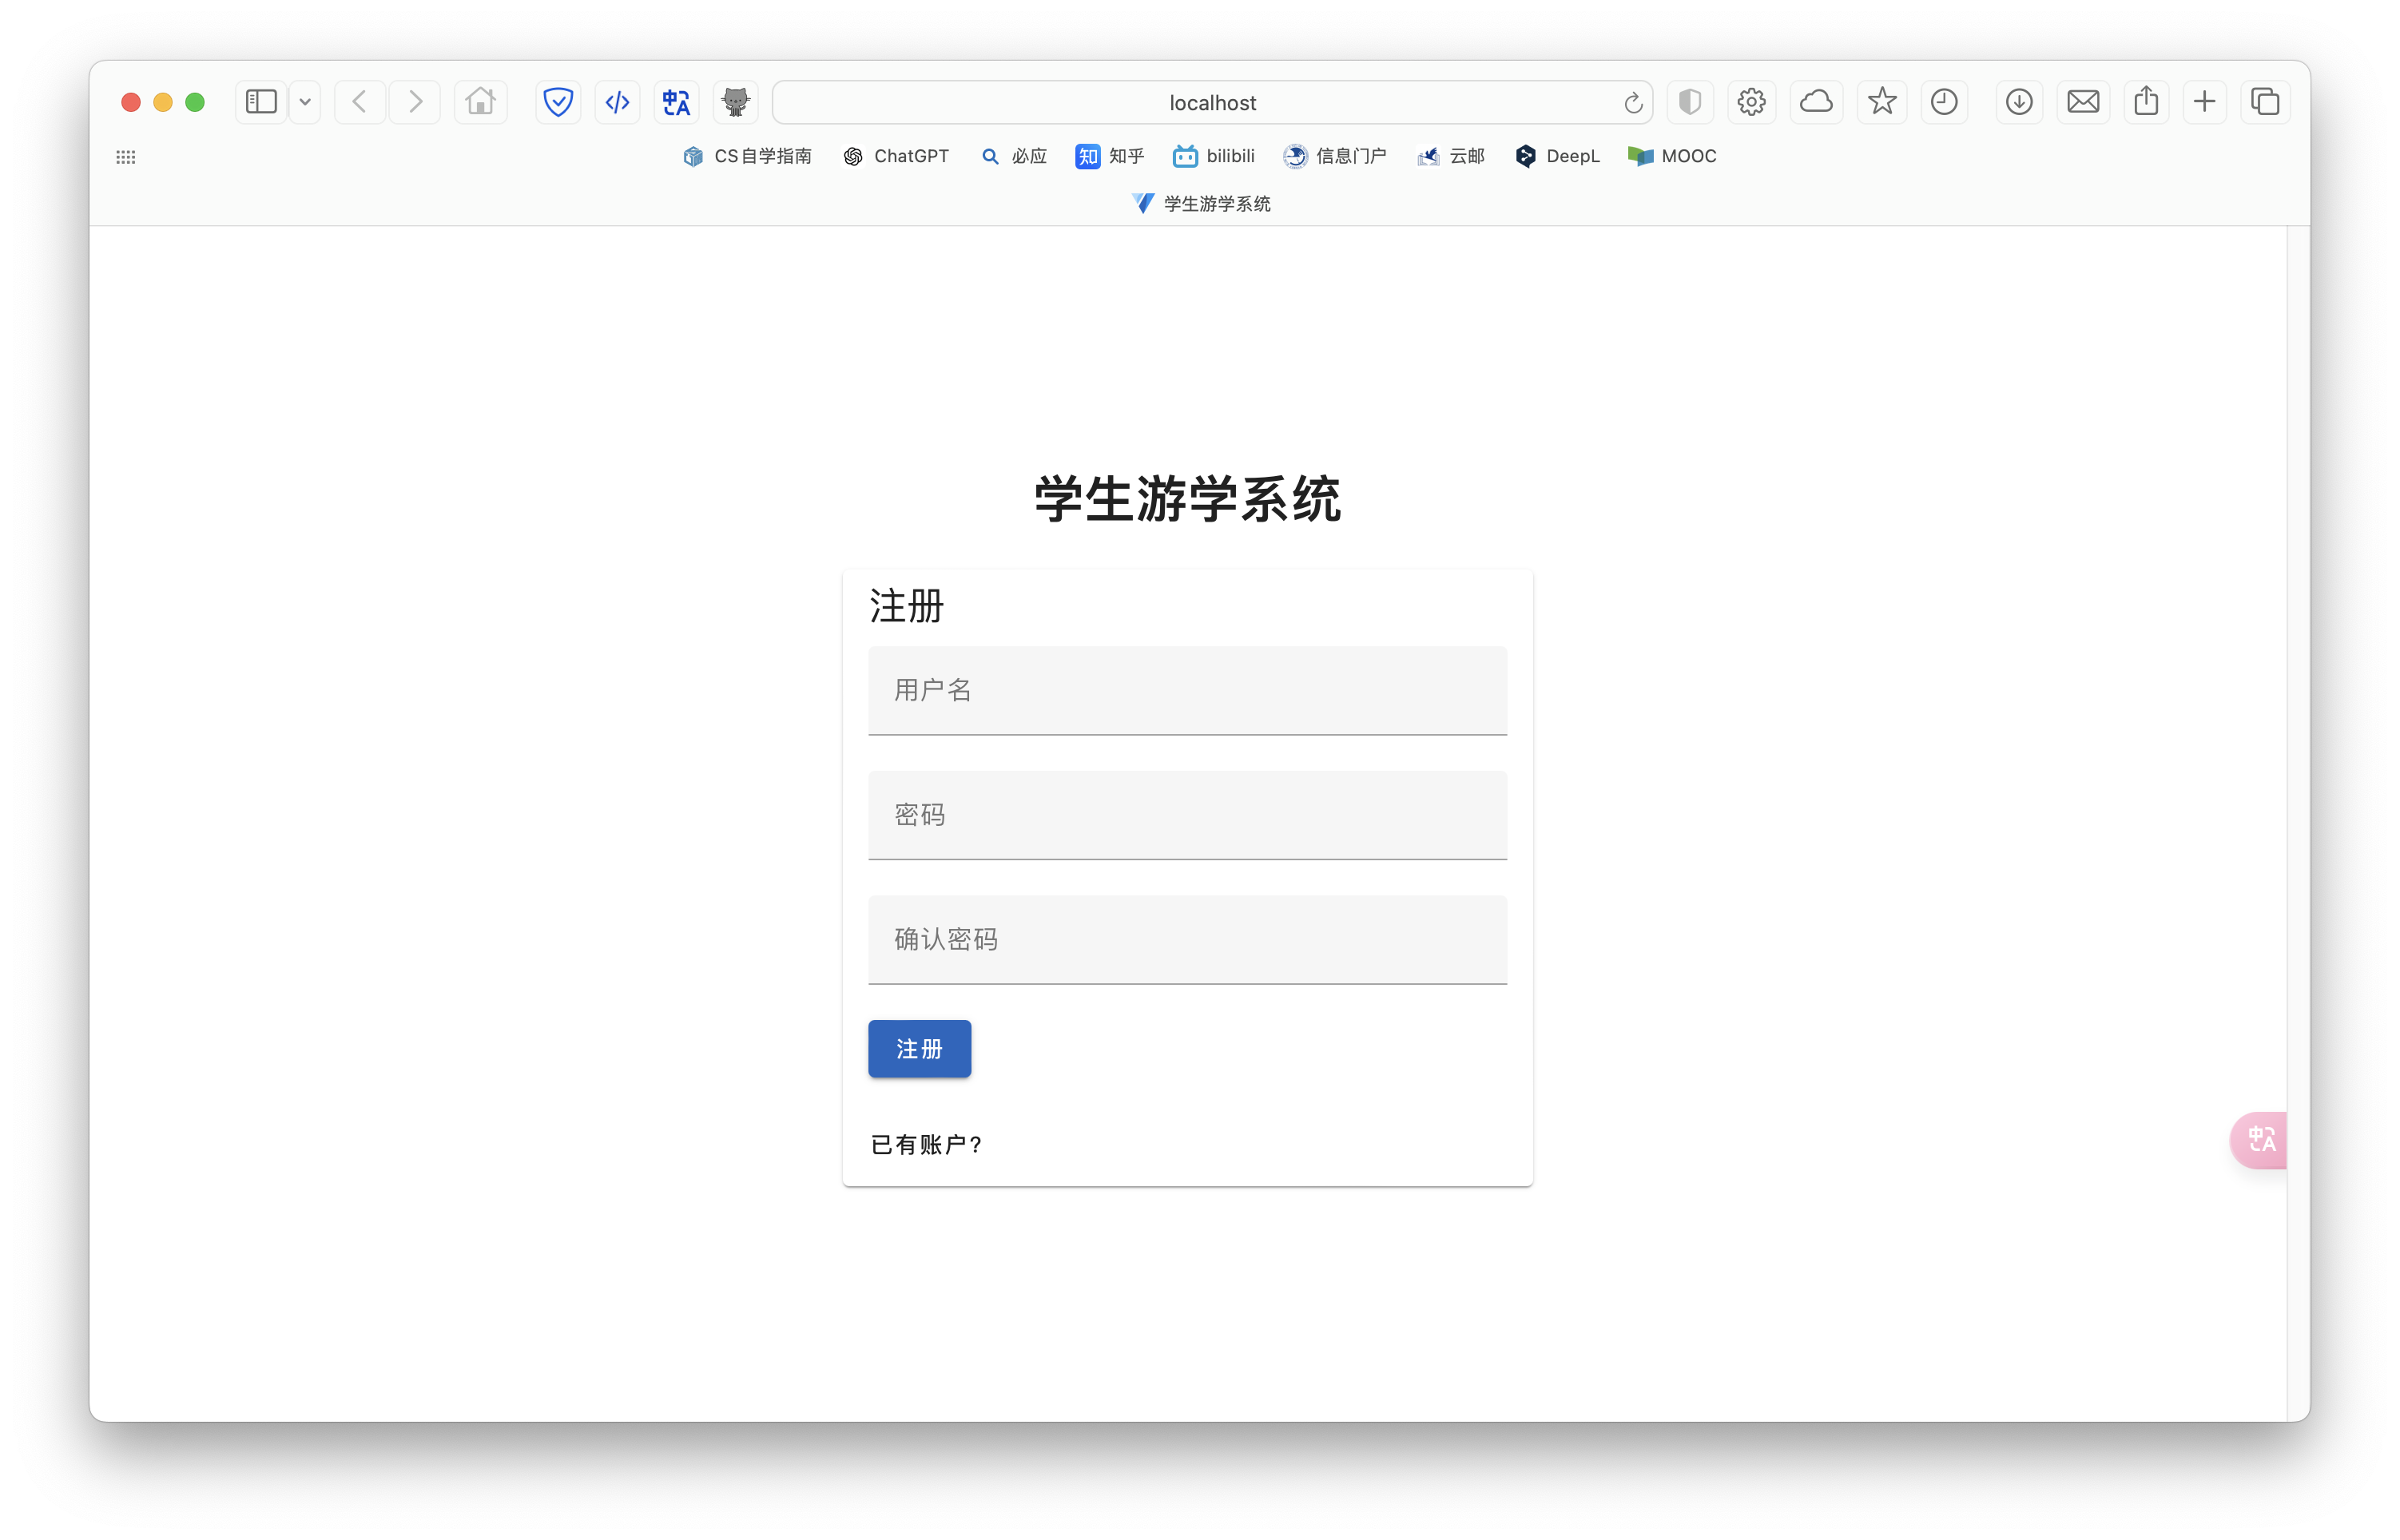
\includegraphics[width=0.85\textwidth]{figure/regist.png}
    \caption{注册界面}
\end{figure}

\begin{figure}[htbp]
    \centering
    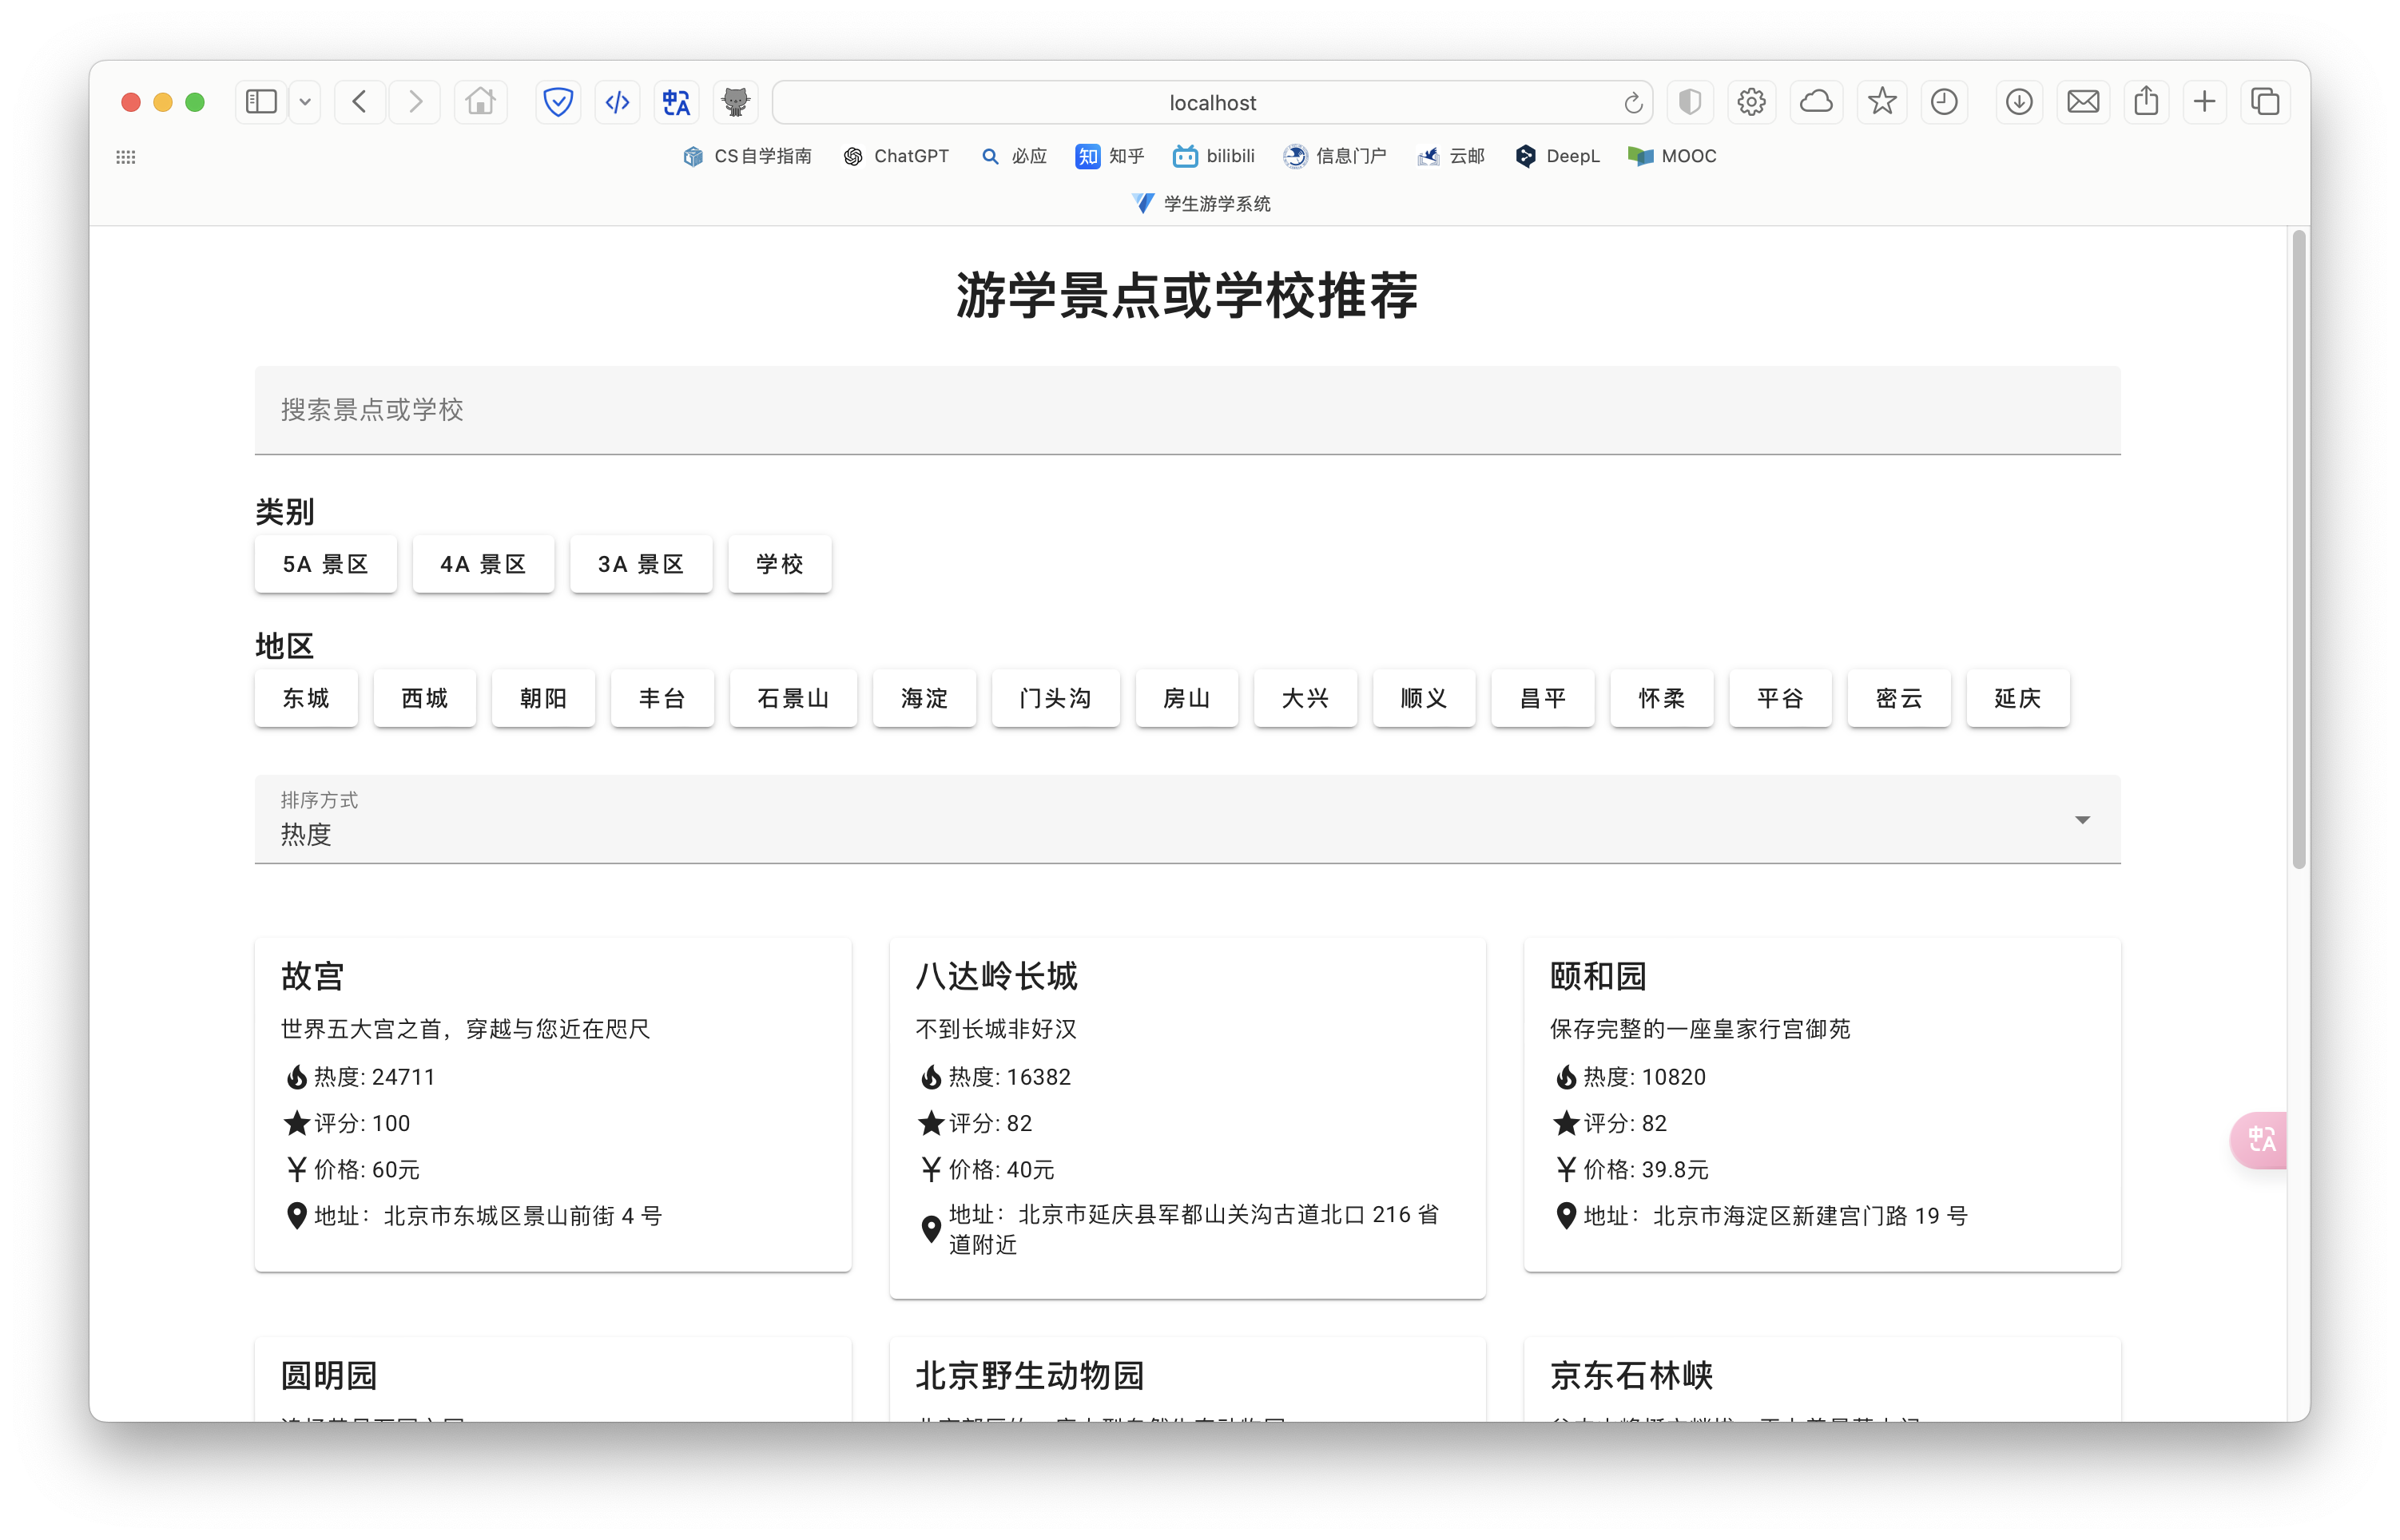
\includegraphics[width=0.85\textwidth]{figure/recommand.png}
    \caption{游学推荐界面}
\end{figure}

\begin{figure}[htbp]
    \centering
    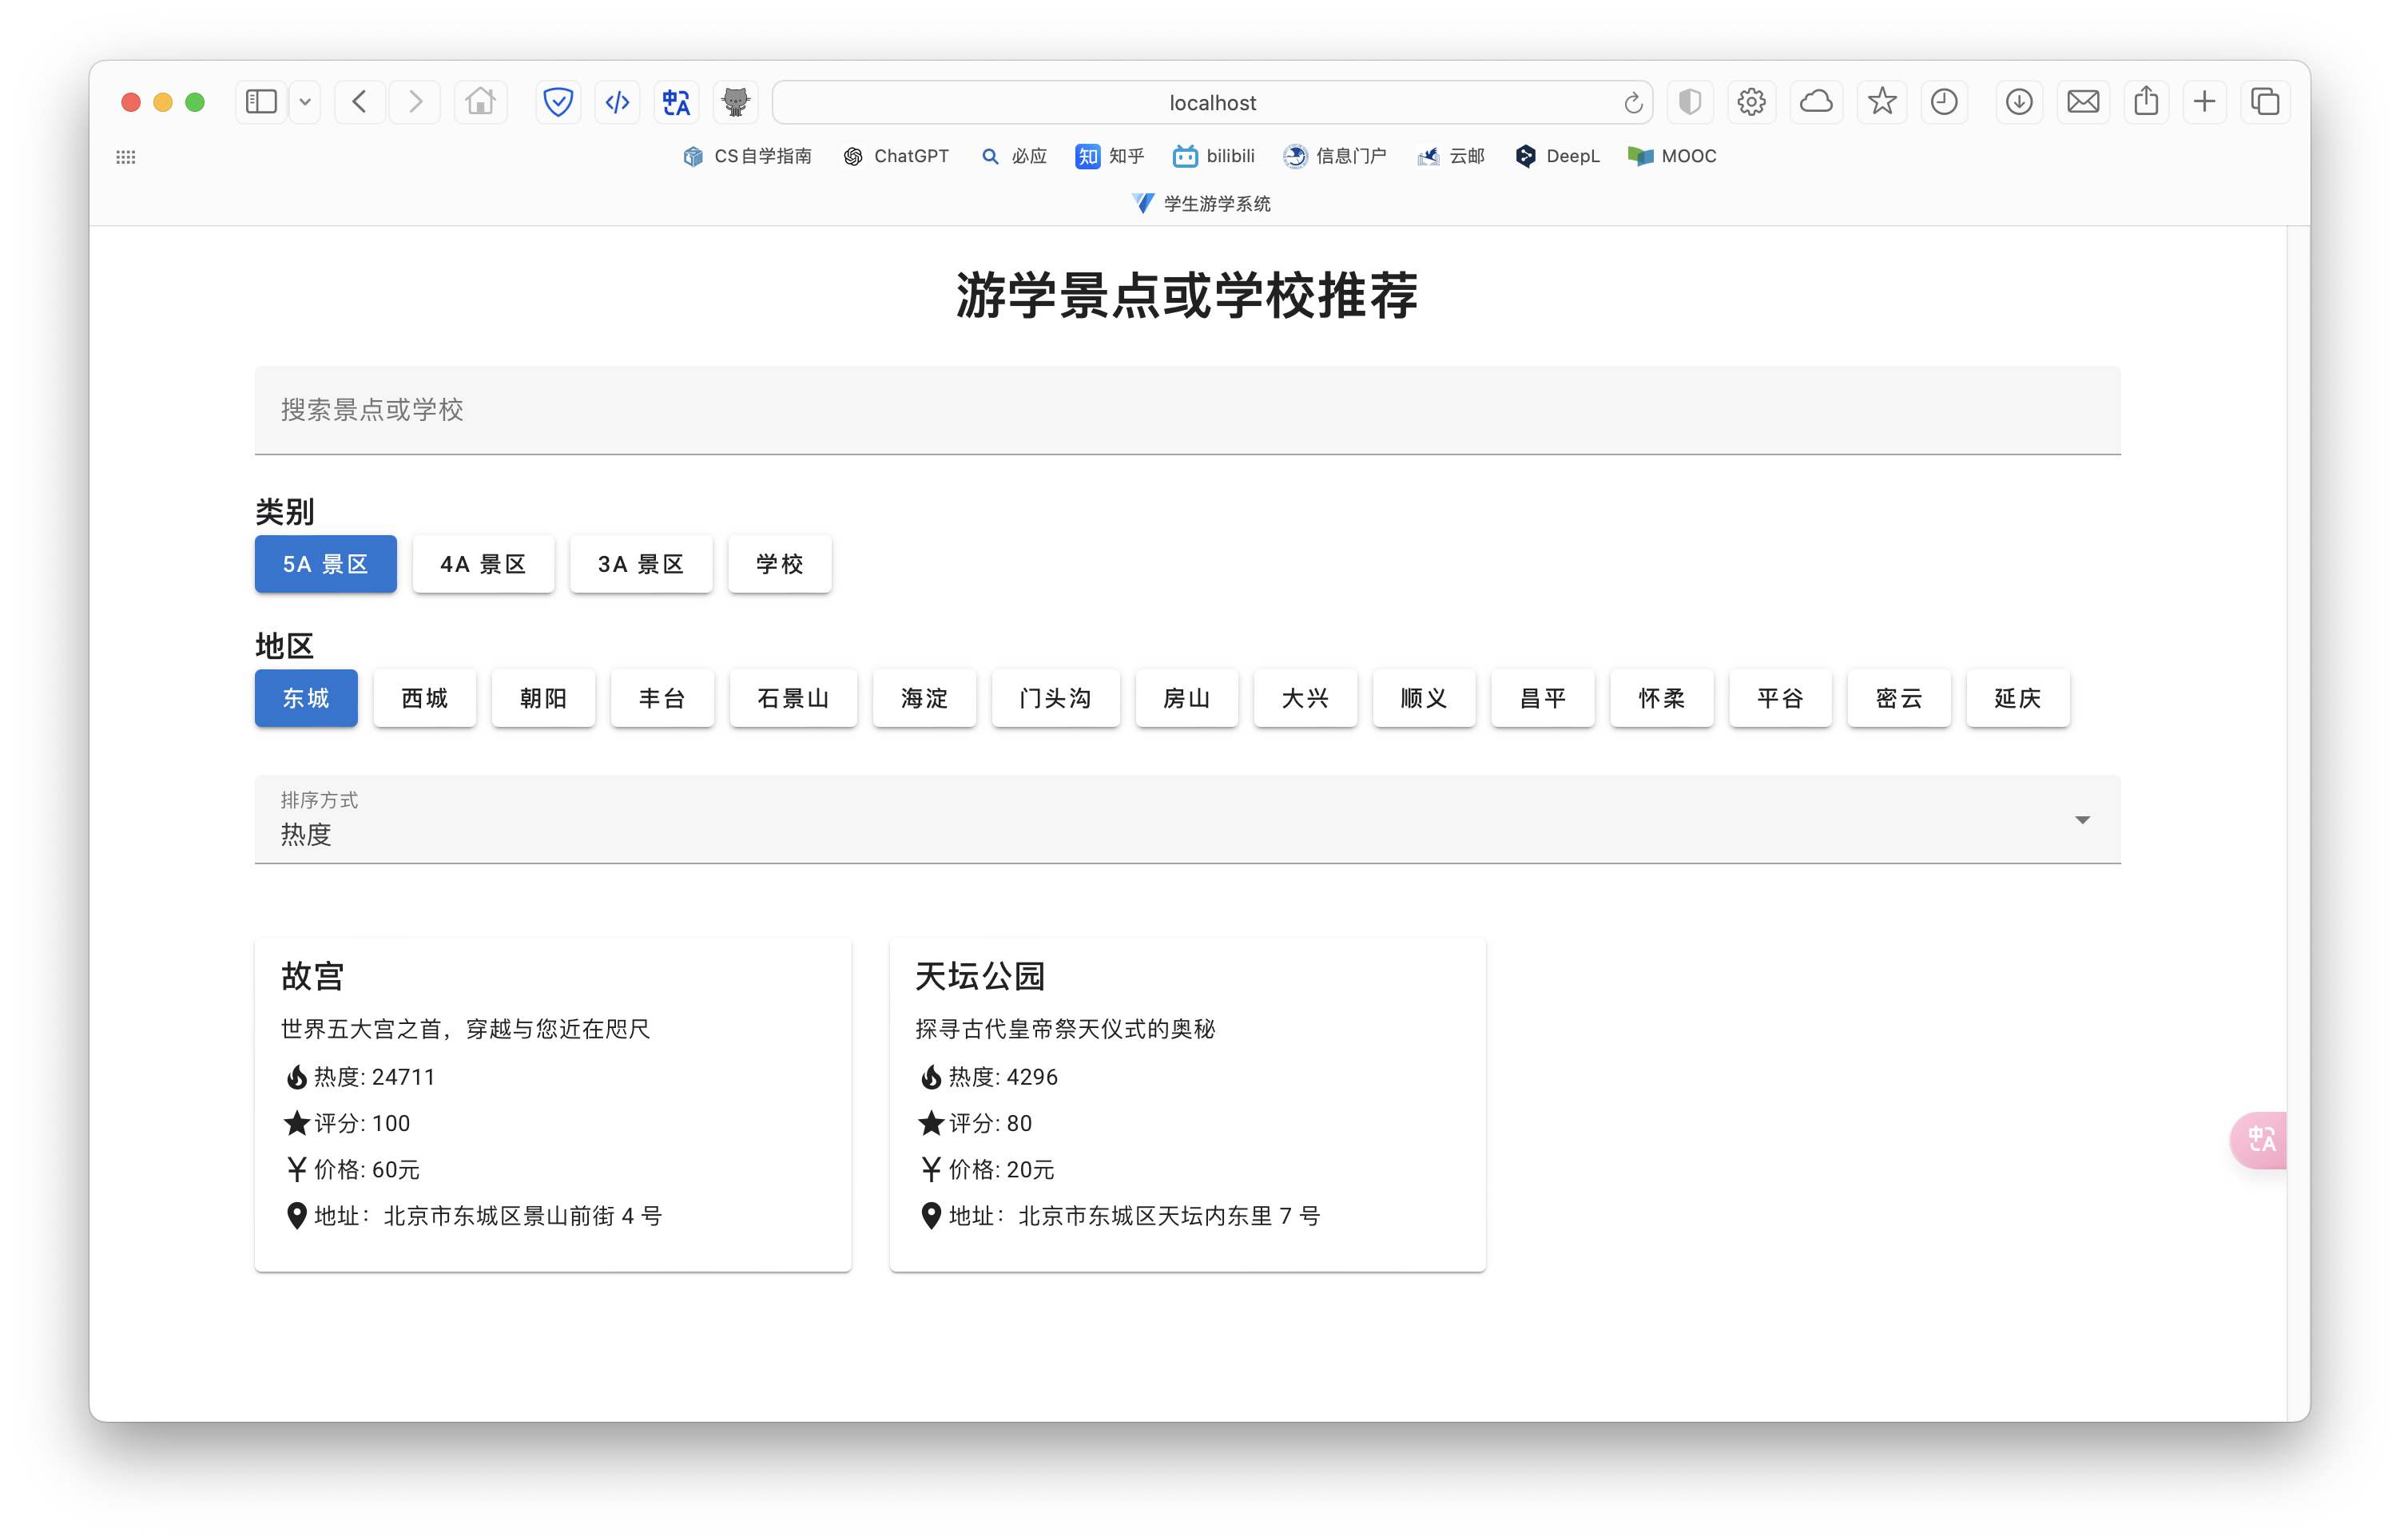
\includegraphics[width=0.85\textwidth]{figure/sort.png}
    \caption{个性化筛选}
\end{figure}

\begin{figure}[htbp]
    \centering
    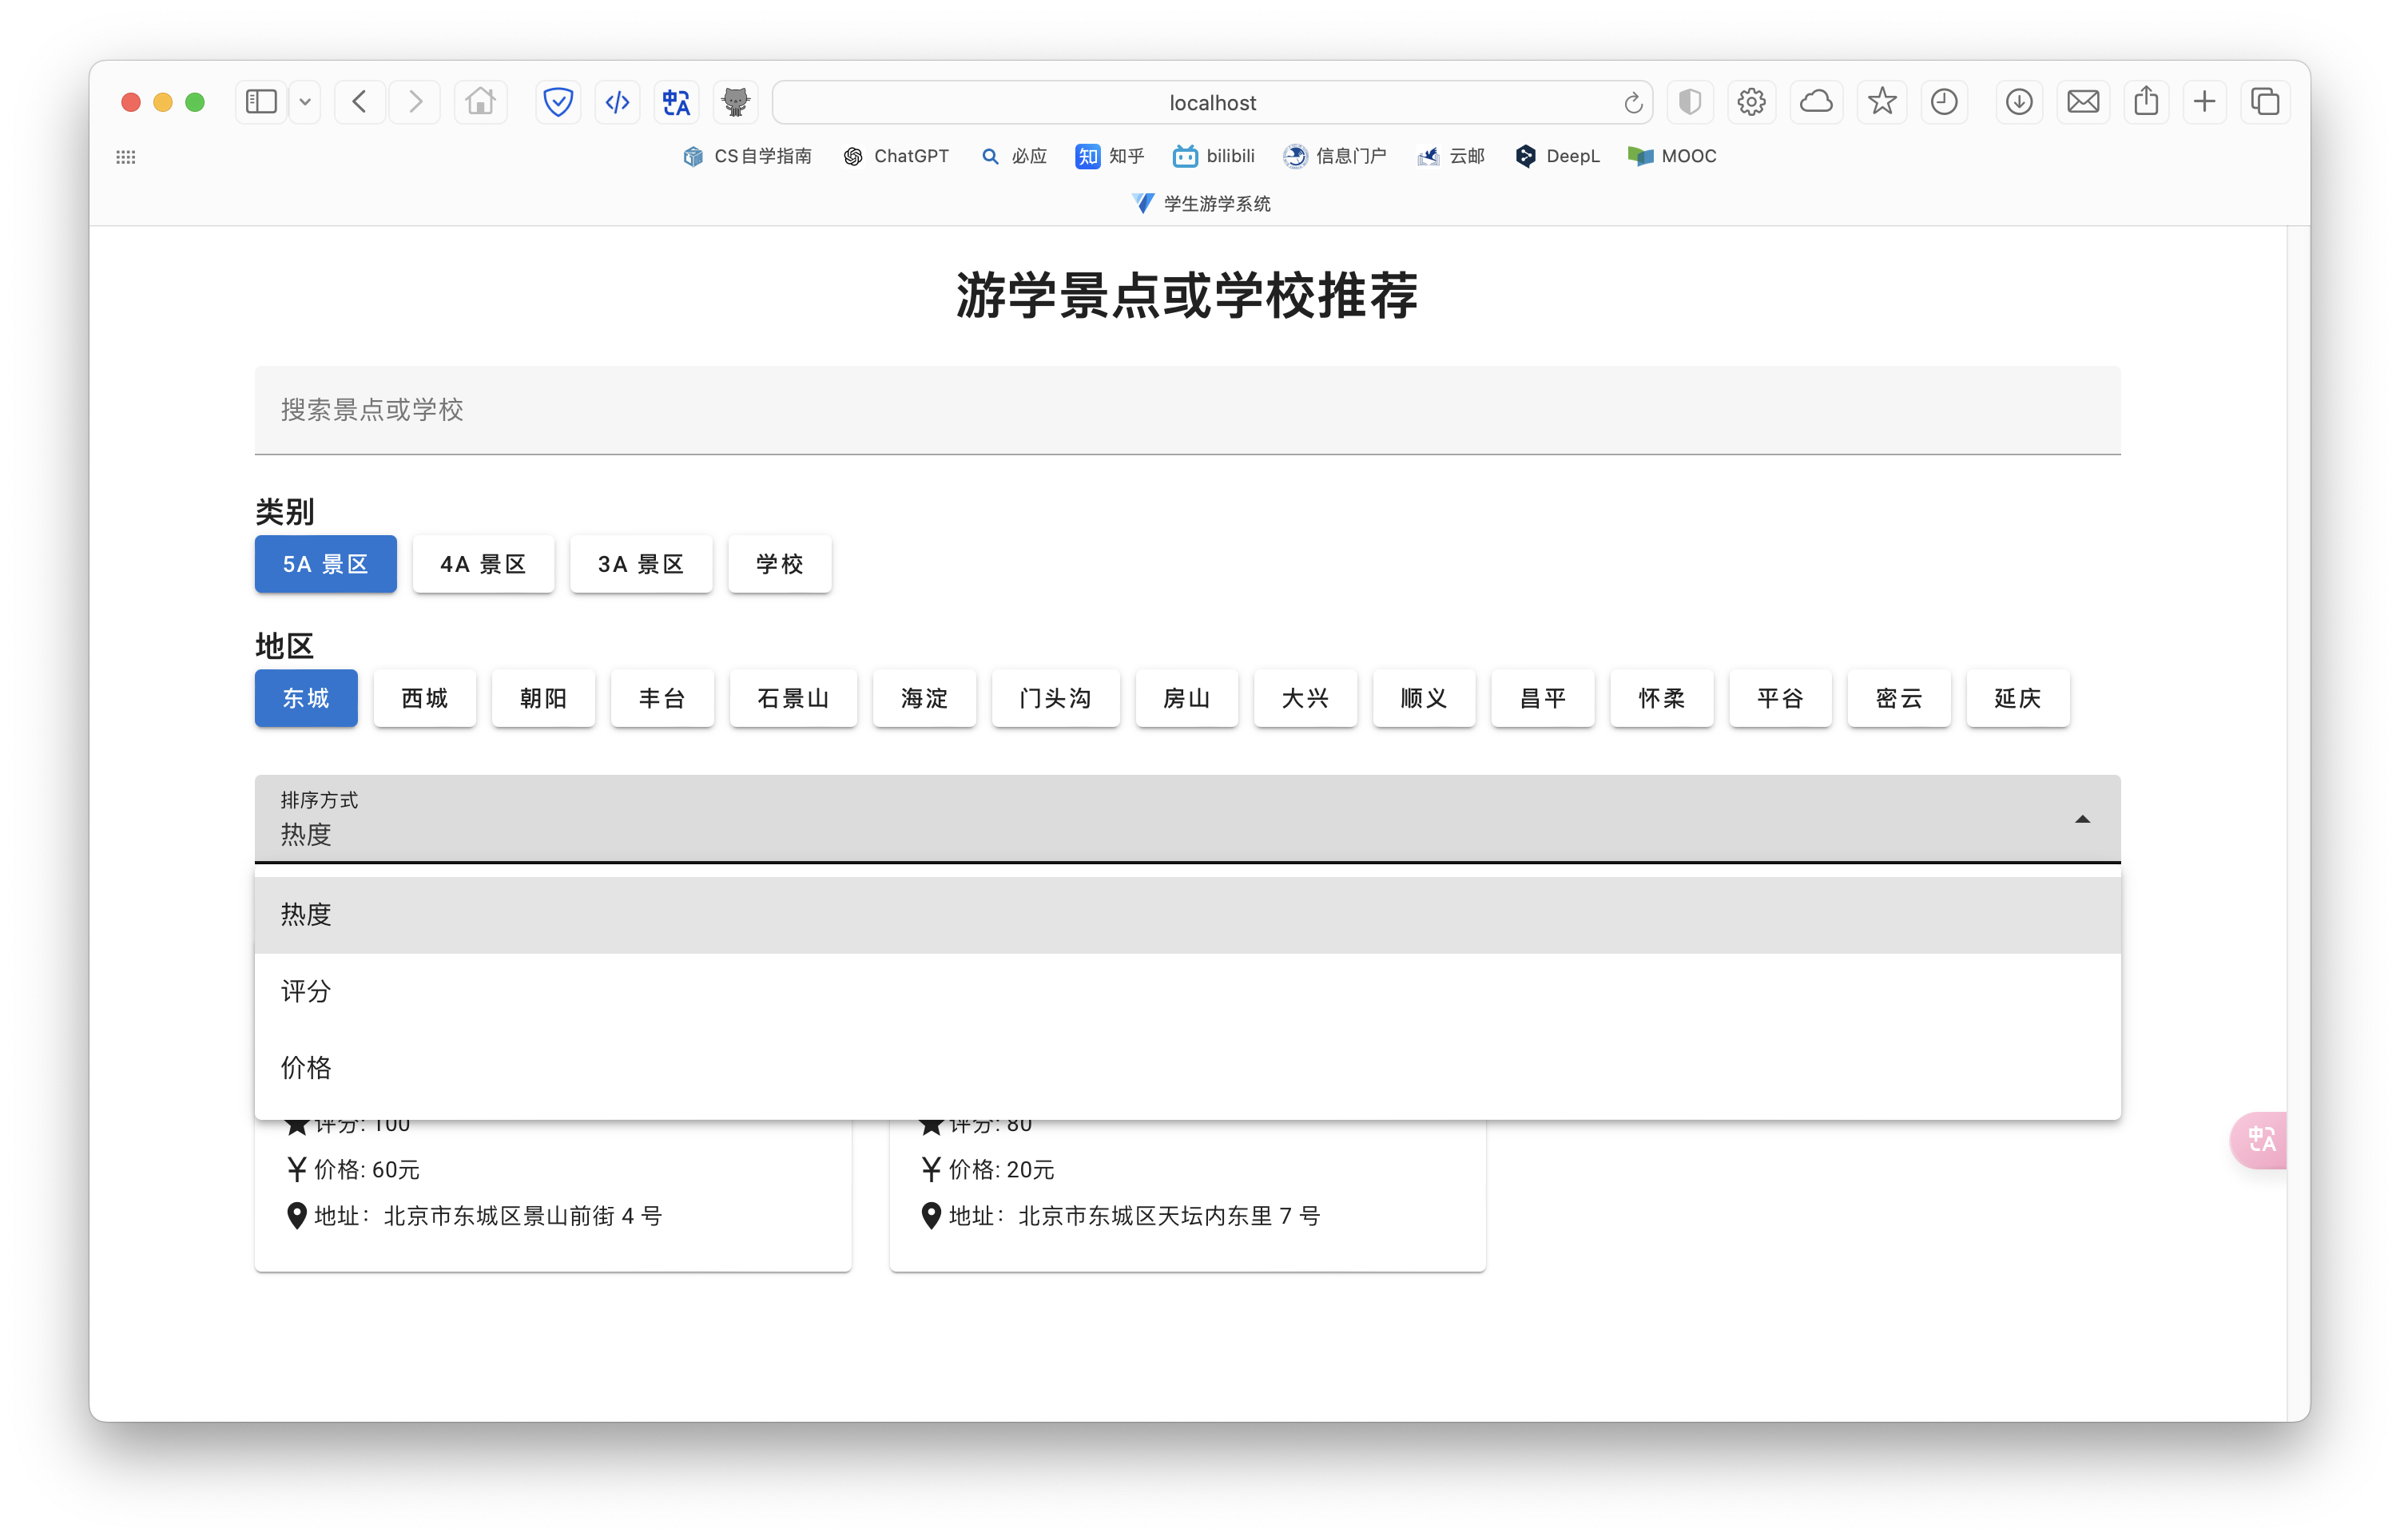
\includegraphics[width=0.85\textwidth]{figure/sortby.png}
    \caption{自定义排序}
\end{figure}

\begin{figure}[htbp]
    \centering
    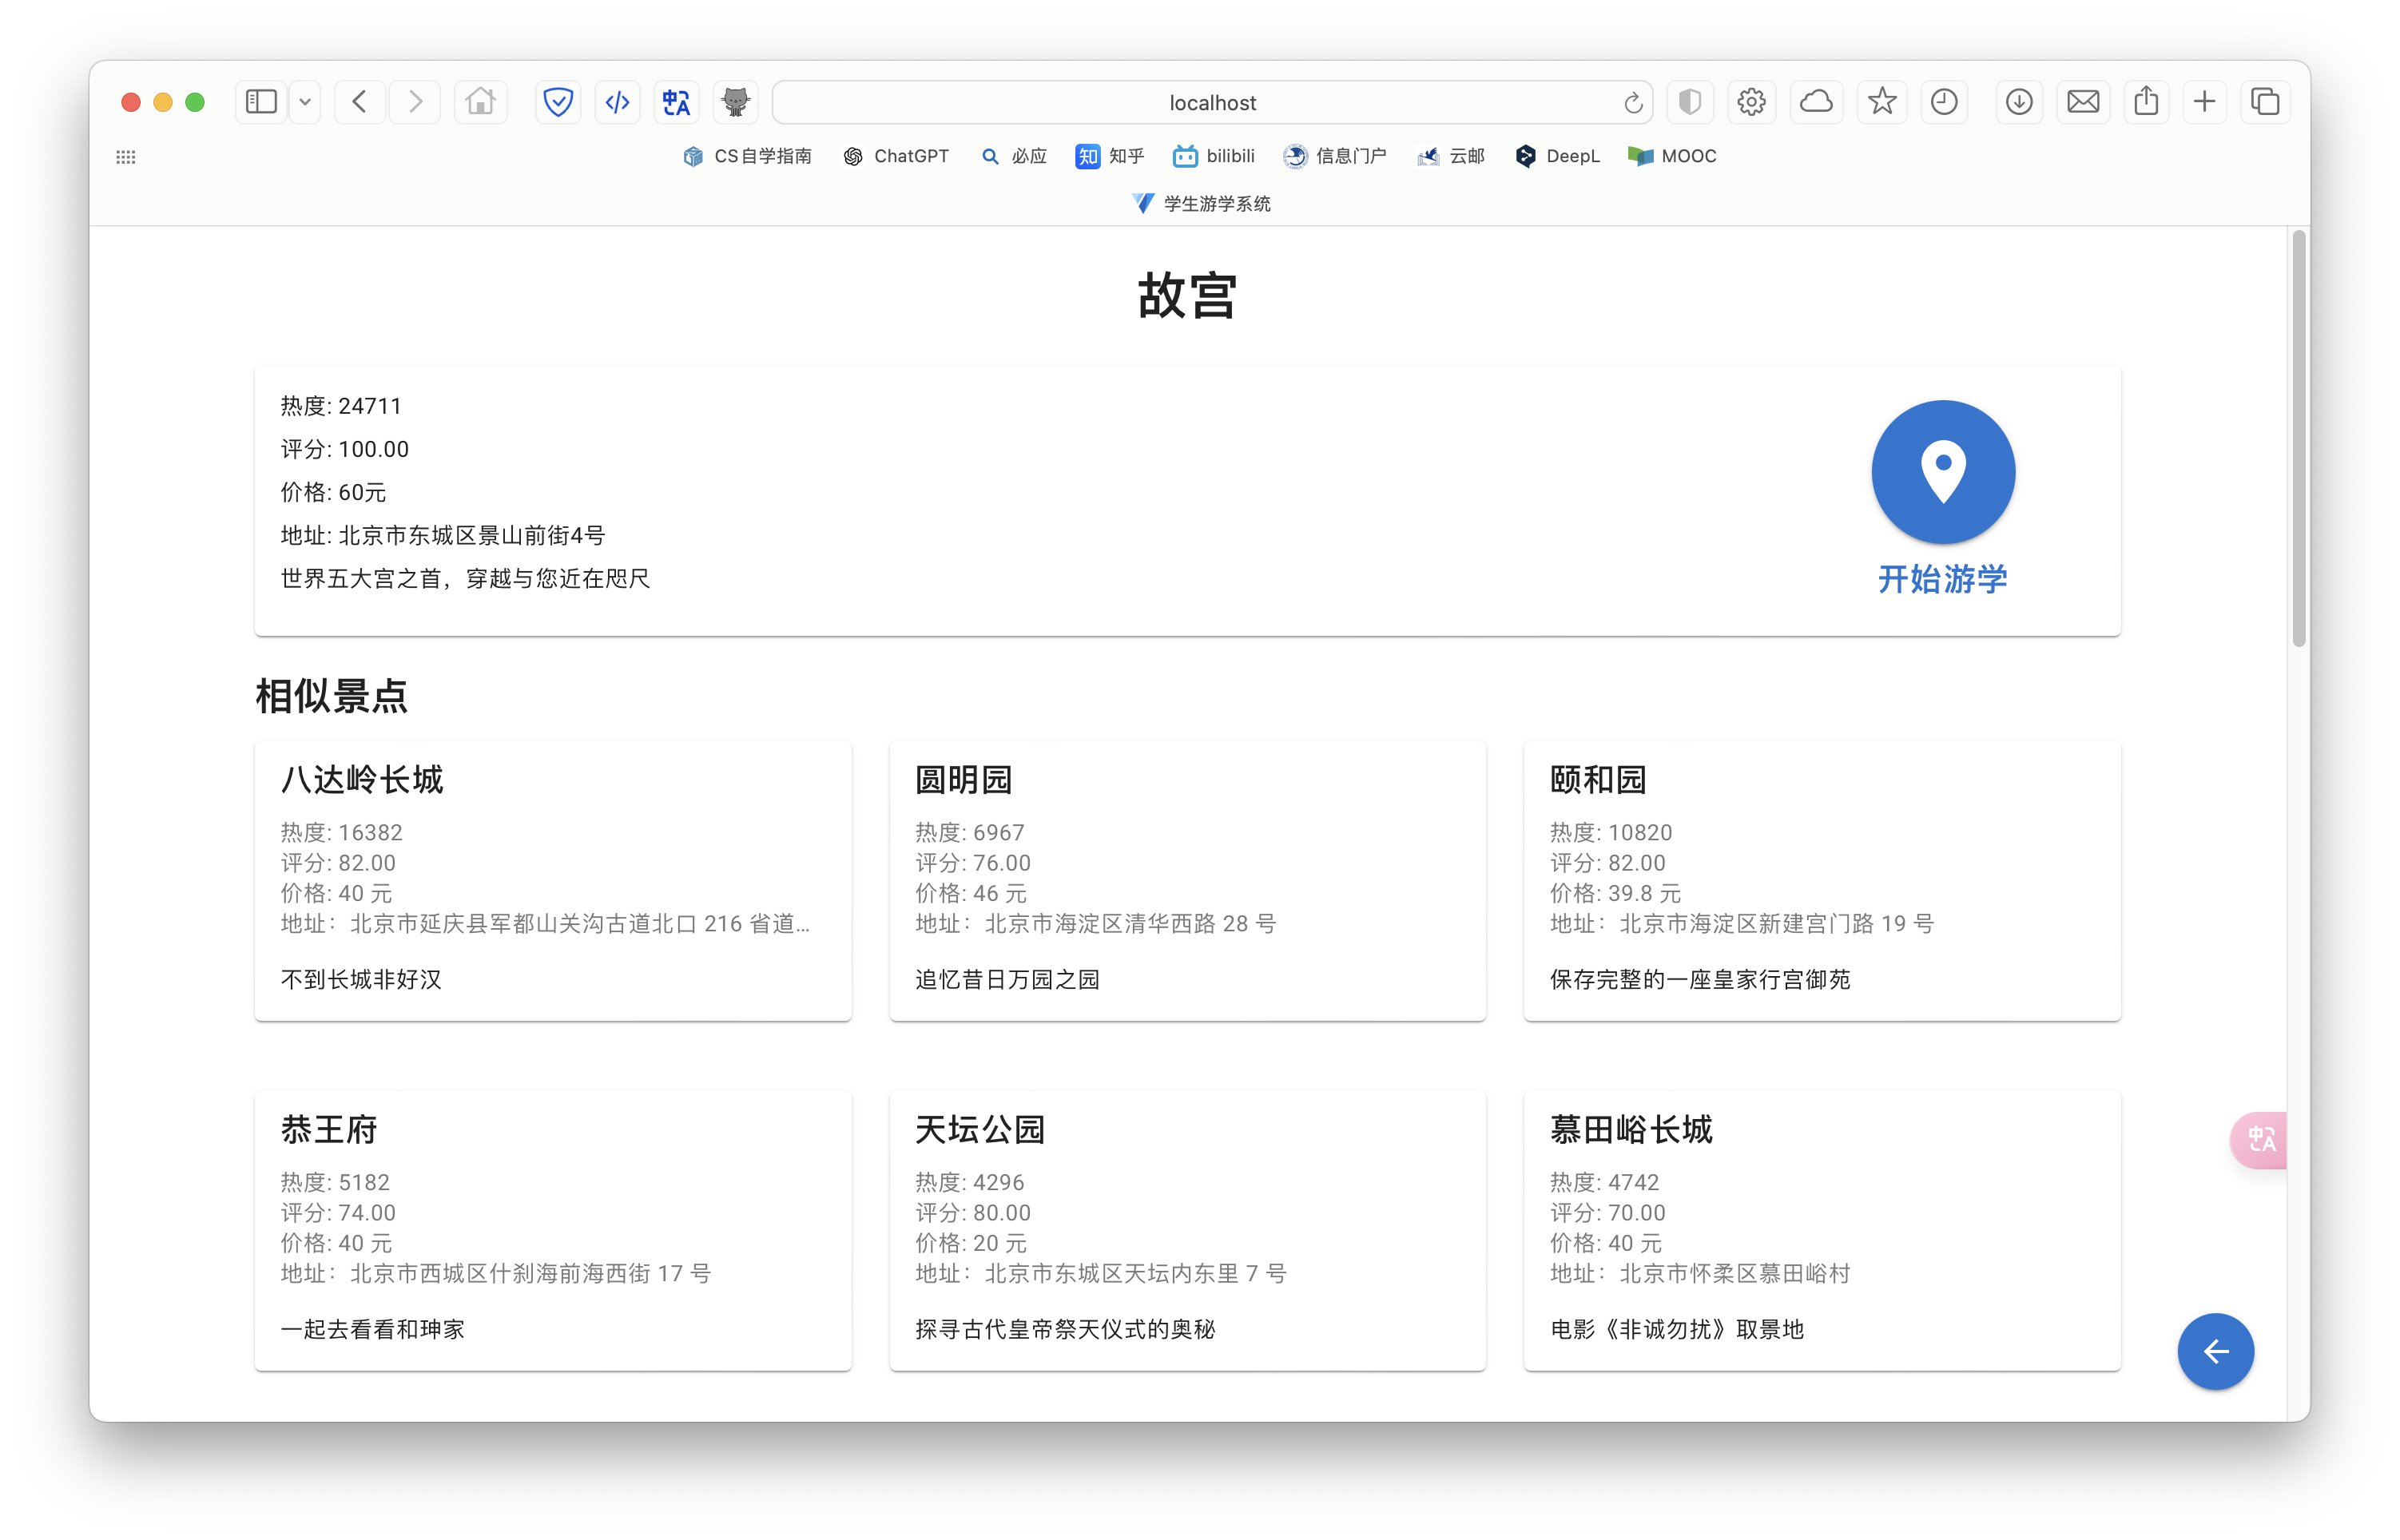
\includegraphics[width=0.85\textwidth]{figure/des.png}
    \caption{景点详情与相似景点推荐}
\end{figure}

\begin{figure}[htbp]
    \centering
    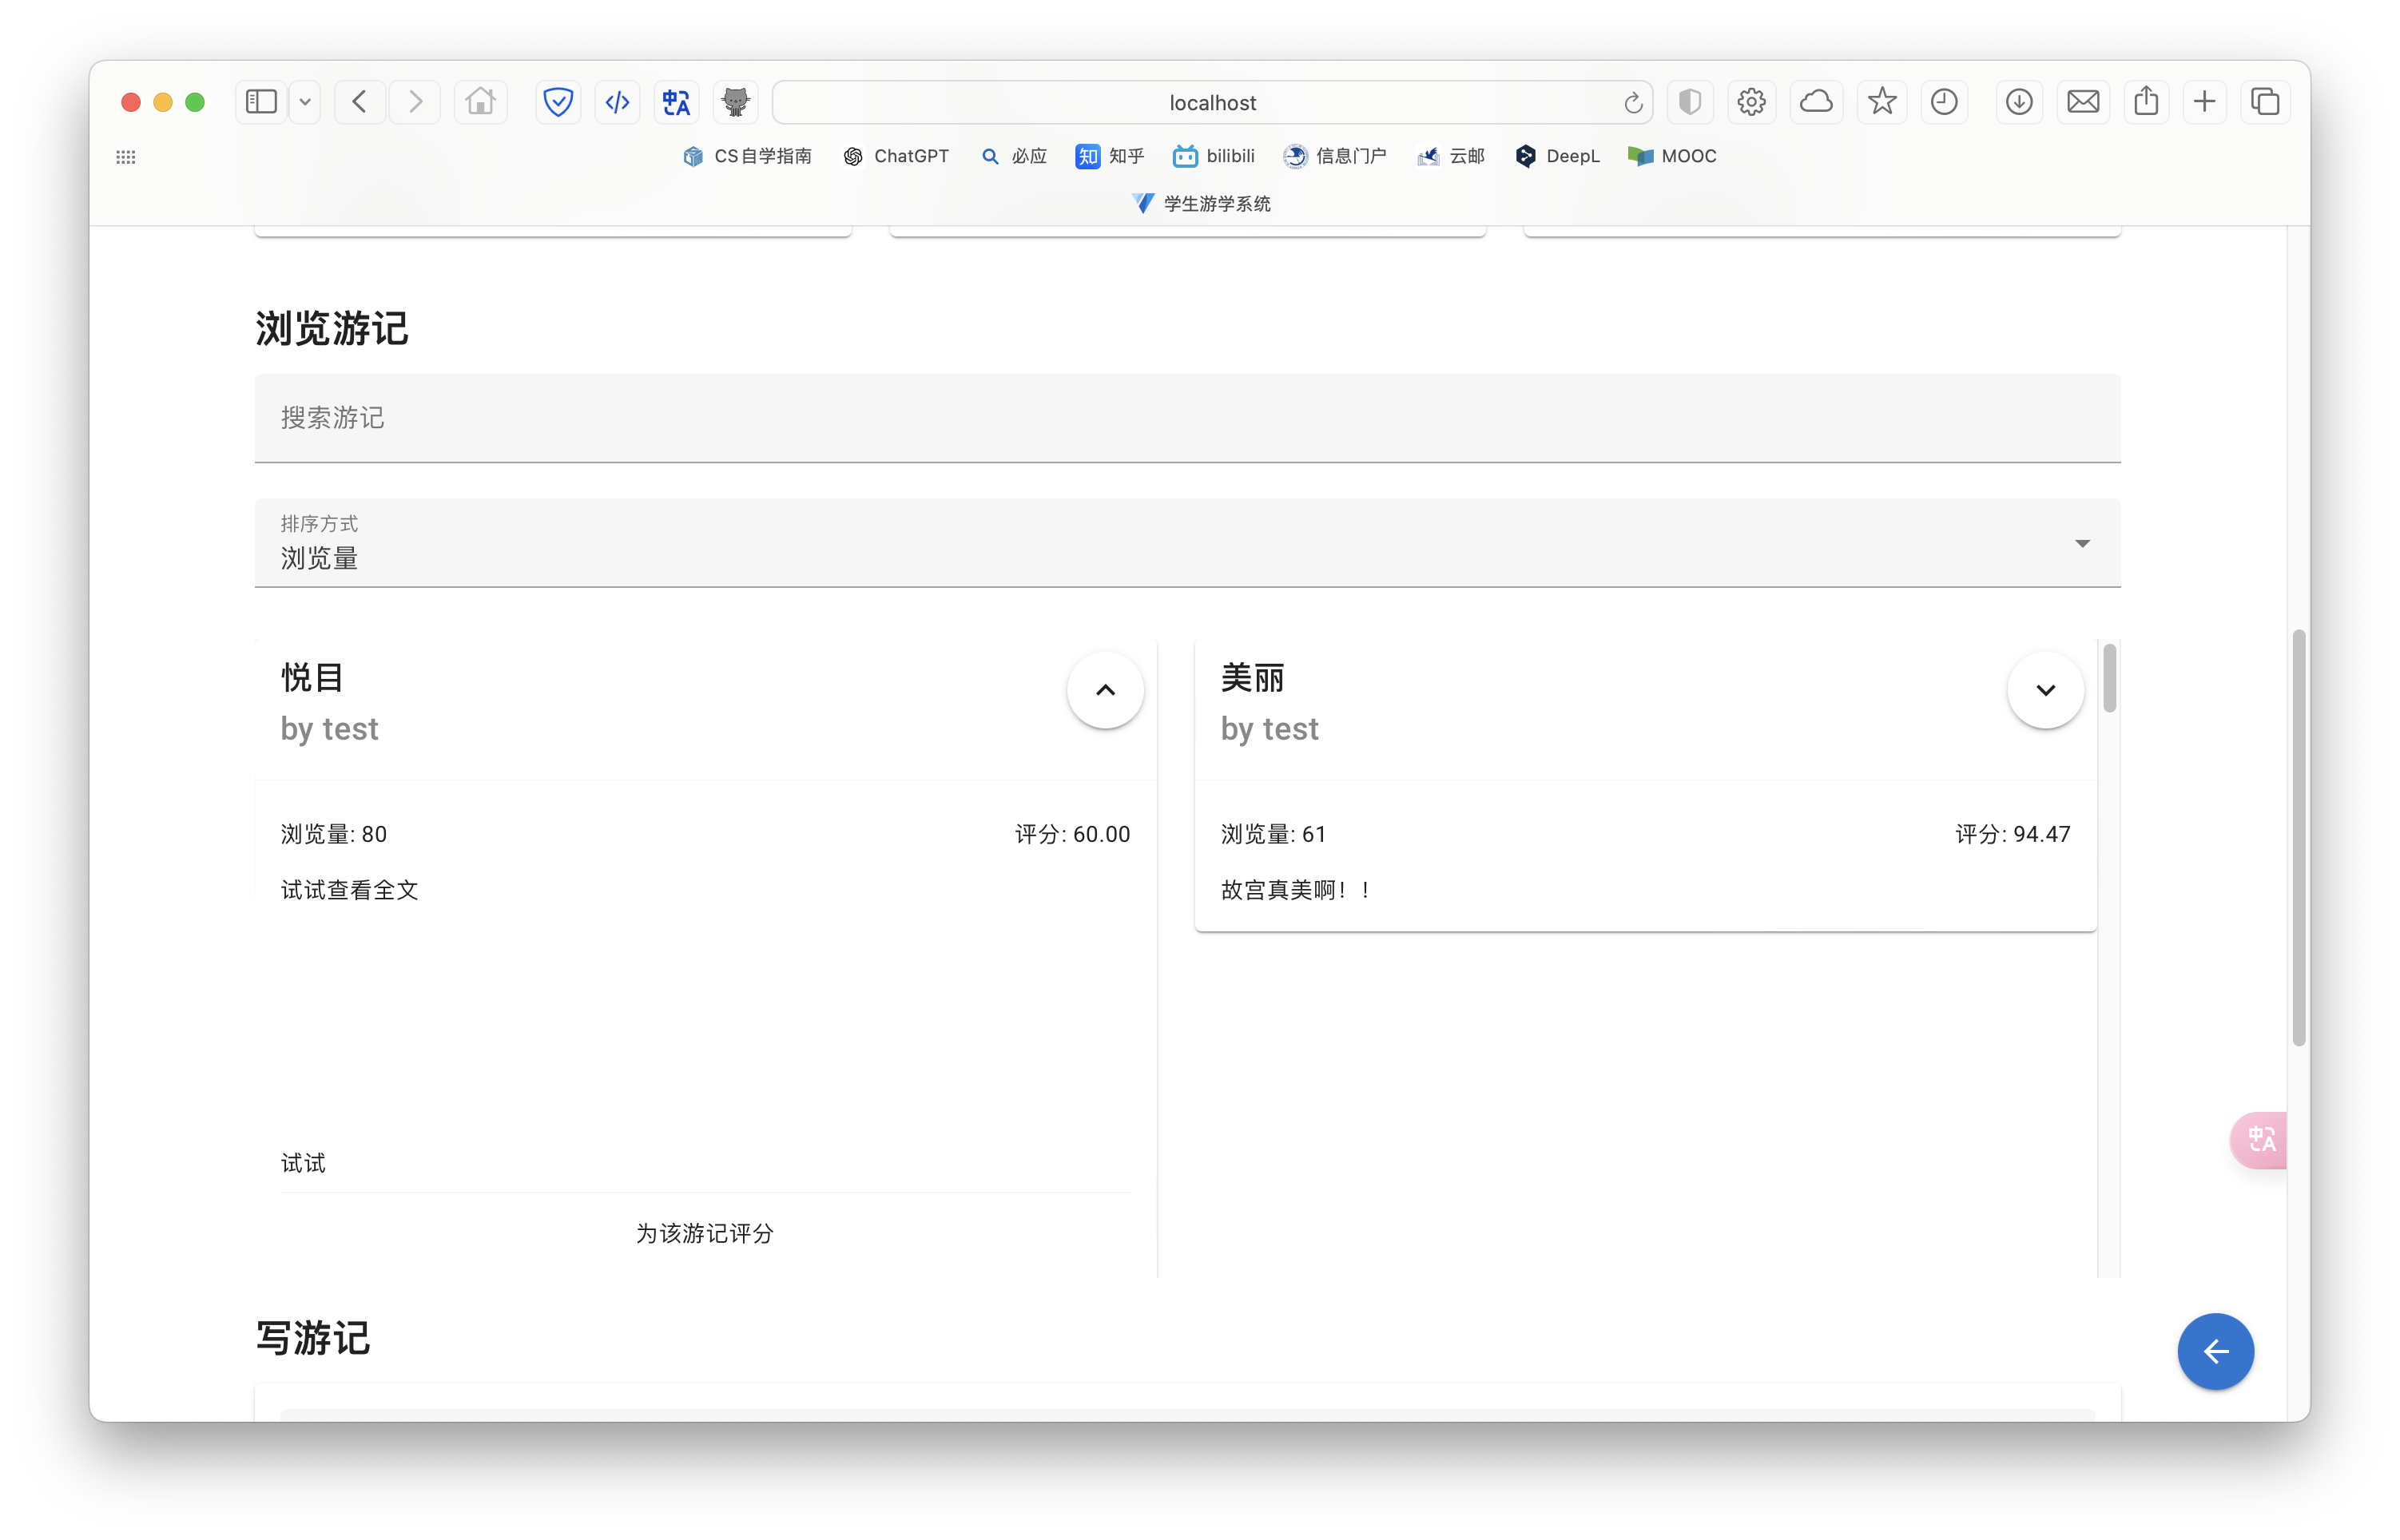
\includegraphics[width=0.85\textwidth]{figure/read.png}
    \caption{浏览游记}
\end{figure}

\begin{figure}[htbp]
    \centering
    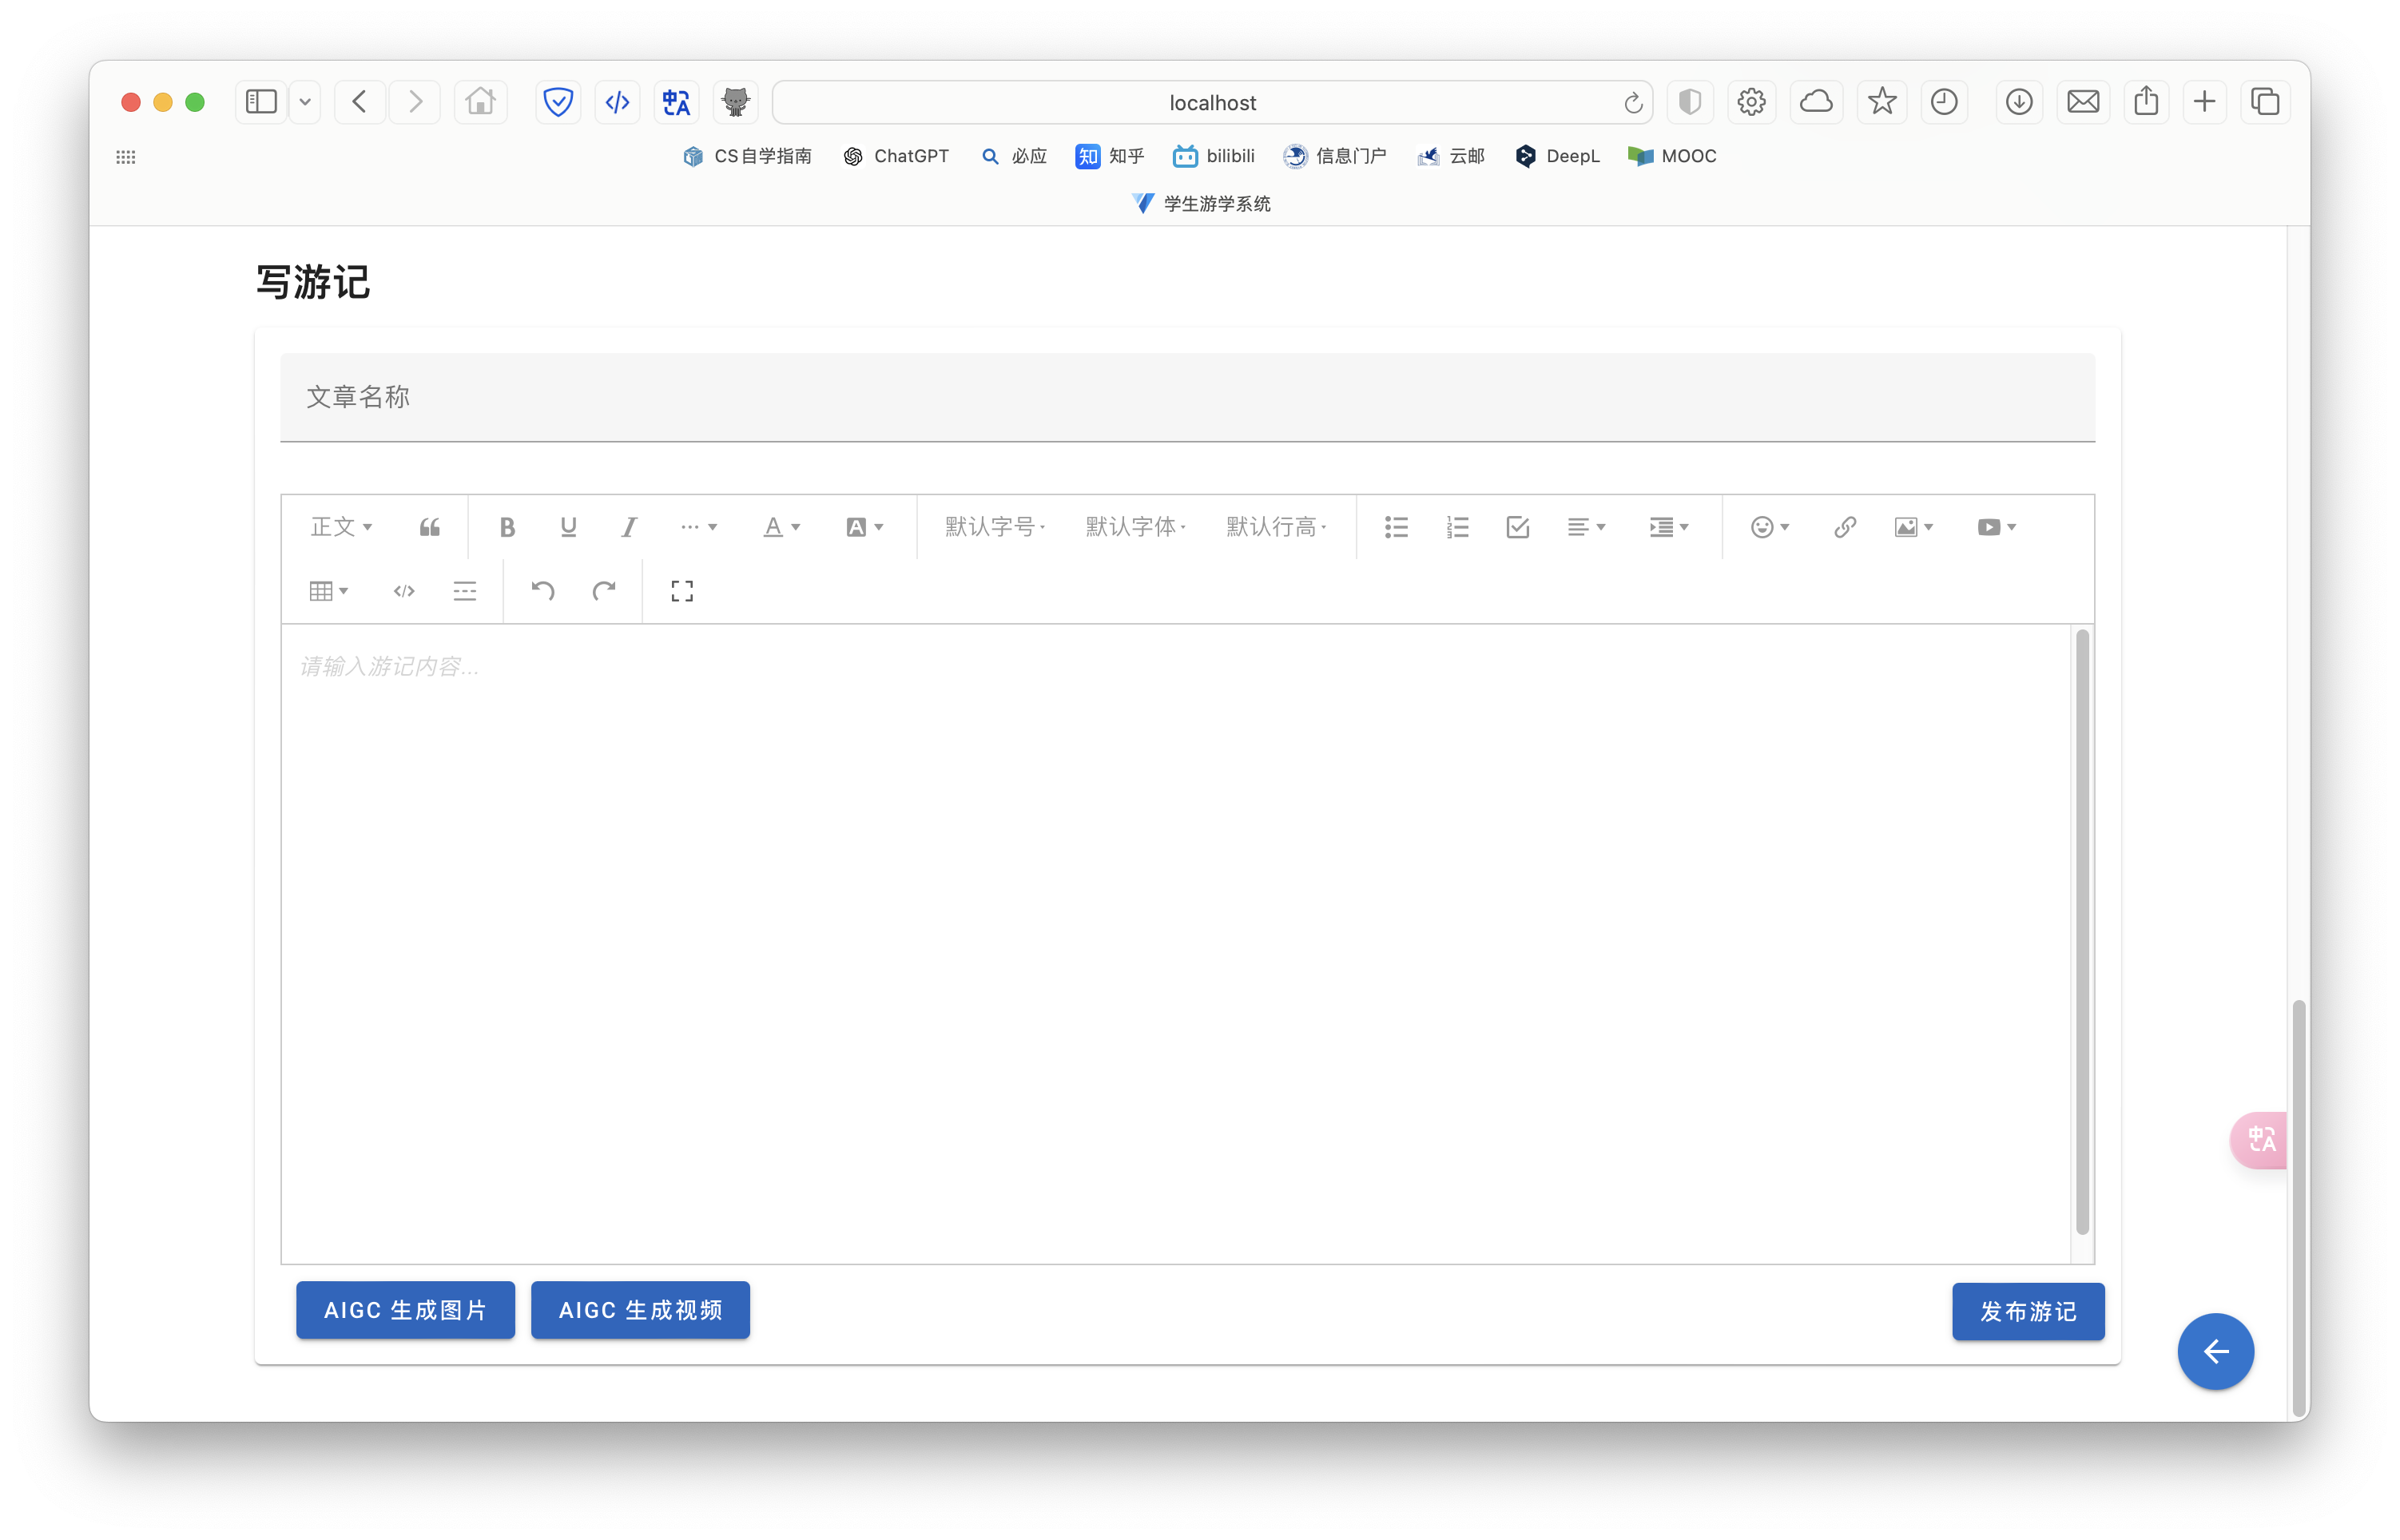
\includegraphics[width=0.85\textwidth]{figure/write.png}
    \caption{写游记及AIGC}
\end{figure}

\begin{figure}[htbp]
    \centering
    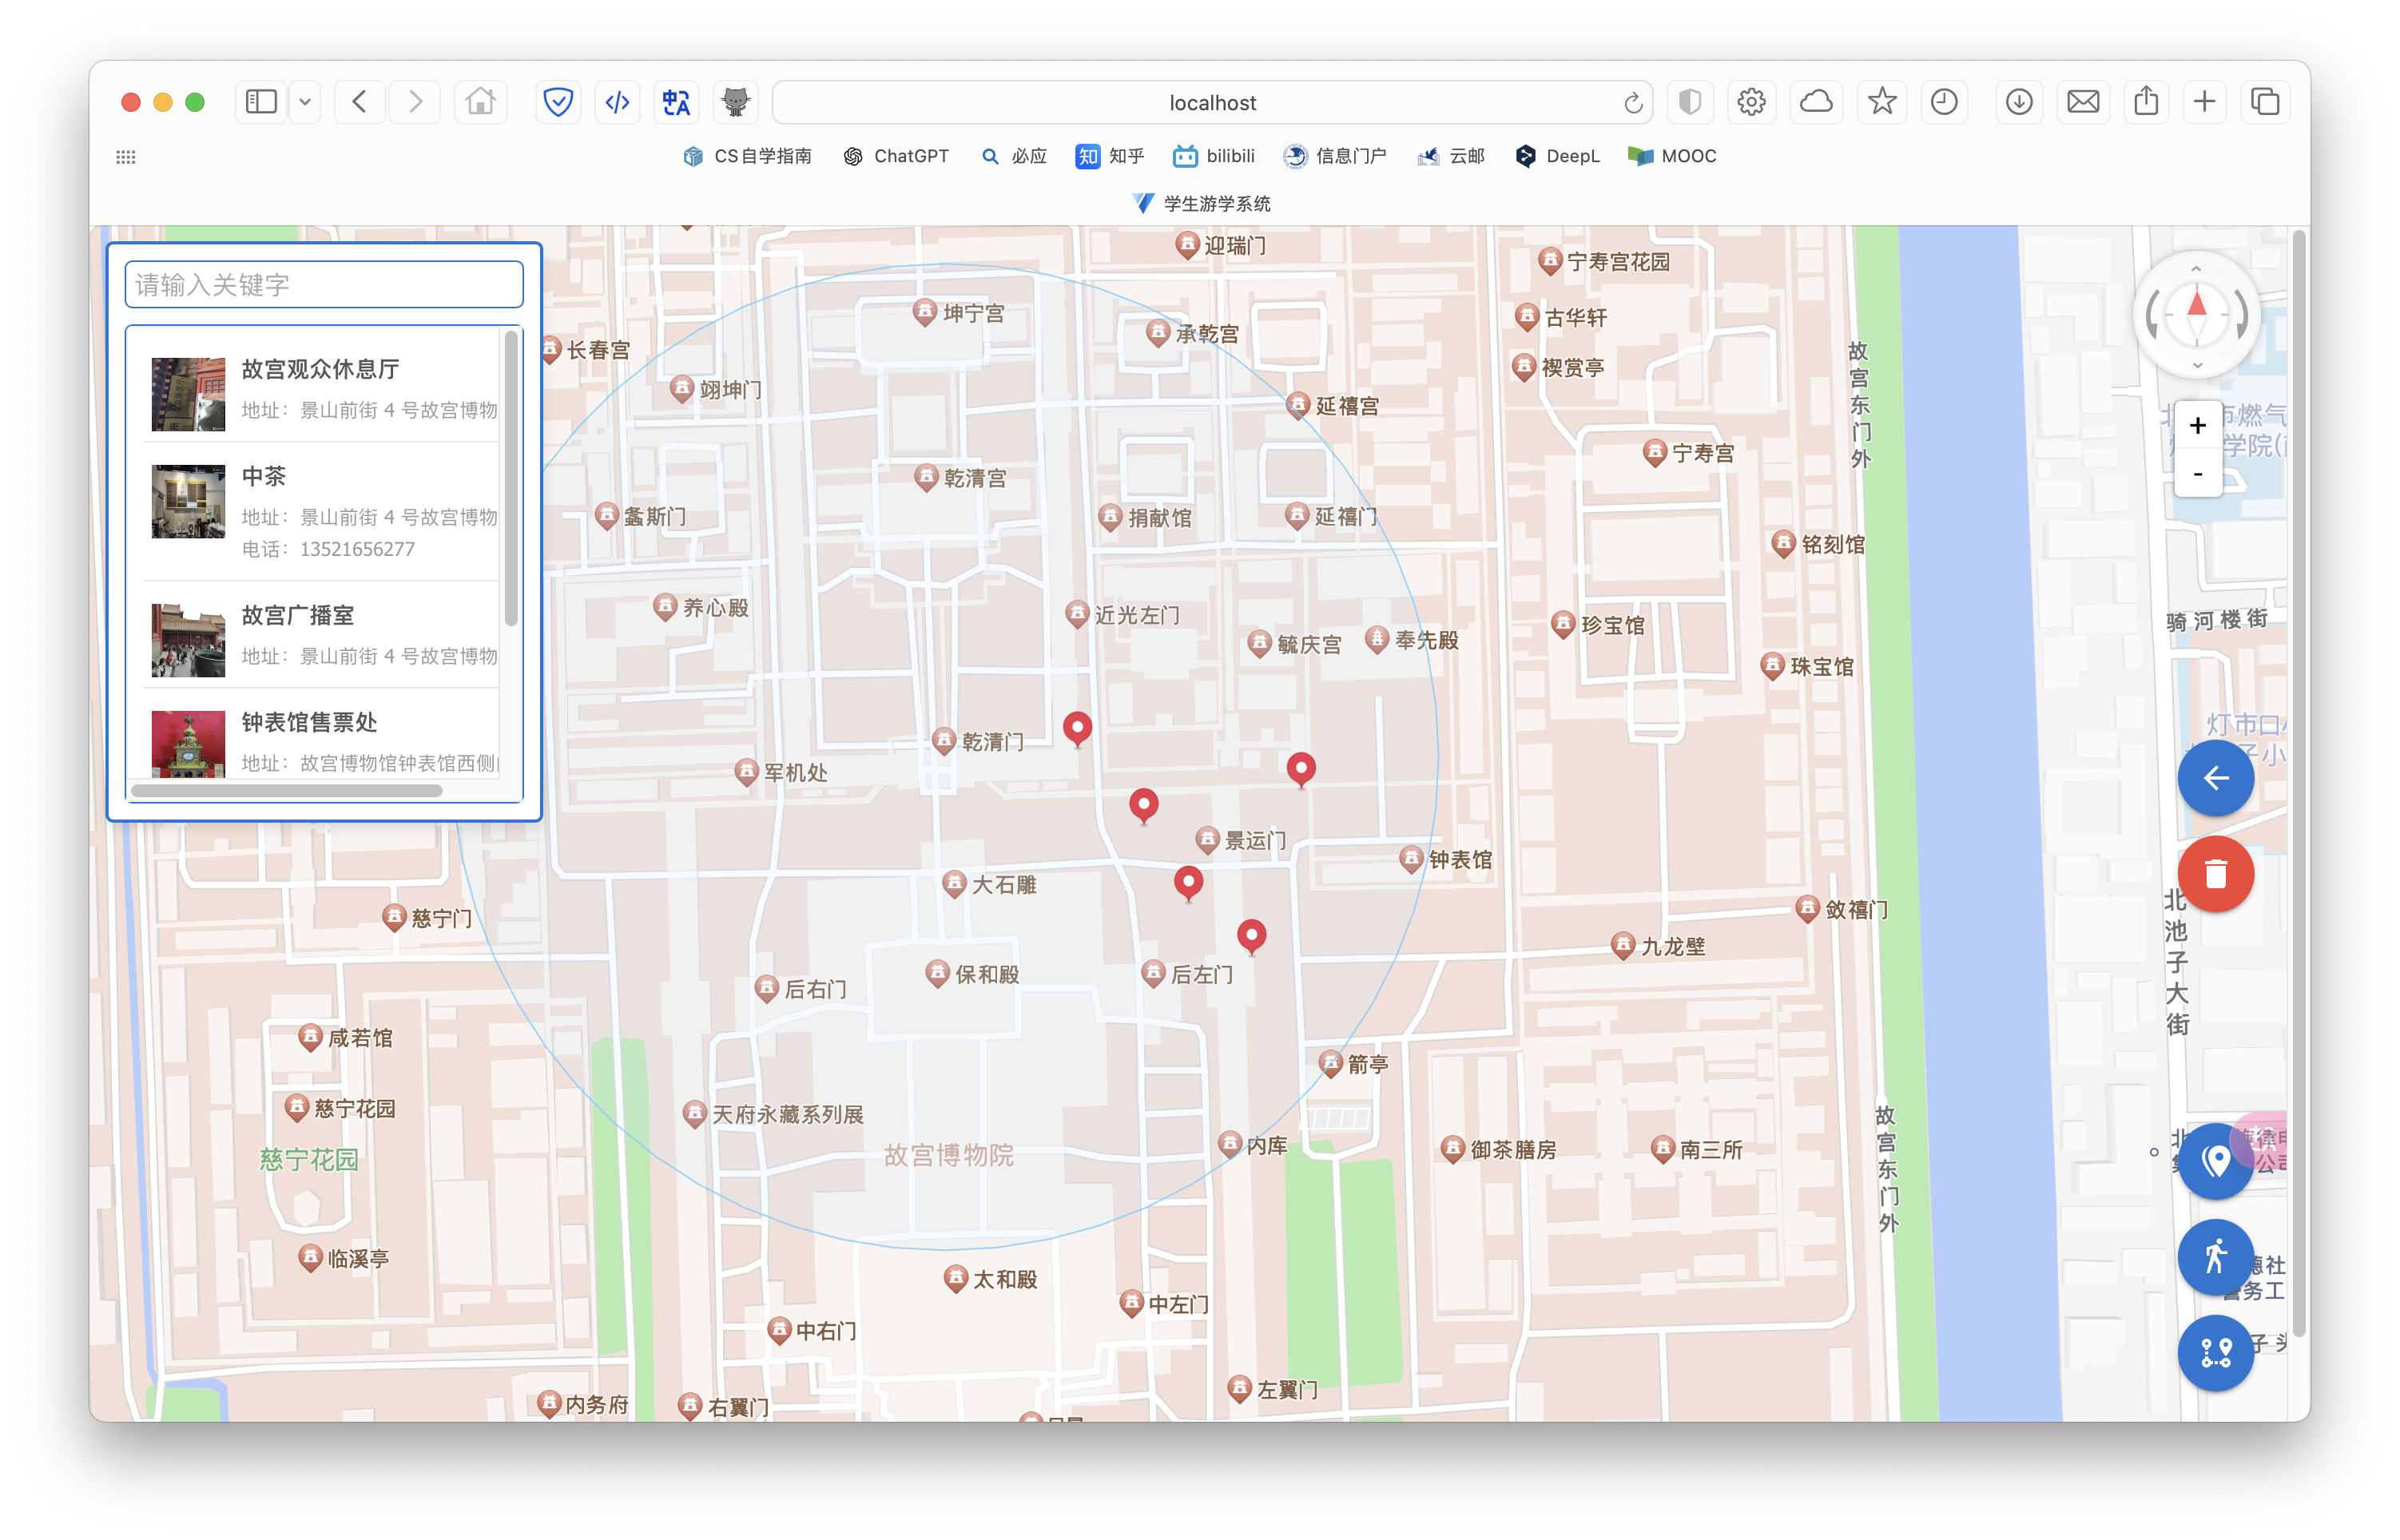
\includegraphics[width=0.85\textwidth]{figure/map.png}
    \caption{地图及周边服务}
\end{figure}

\begin{figure}[htbp]
    \centering
    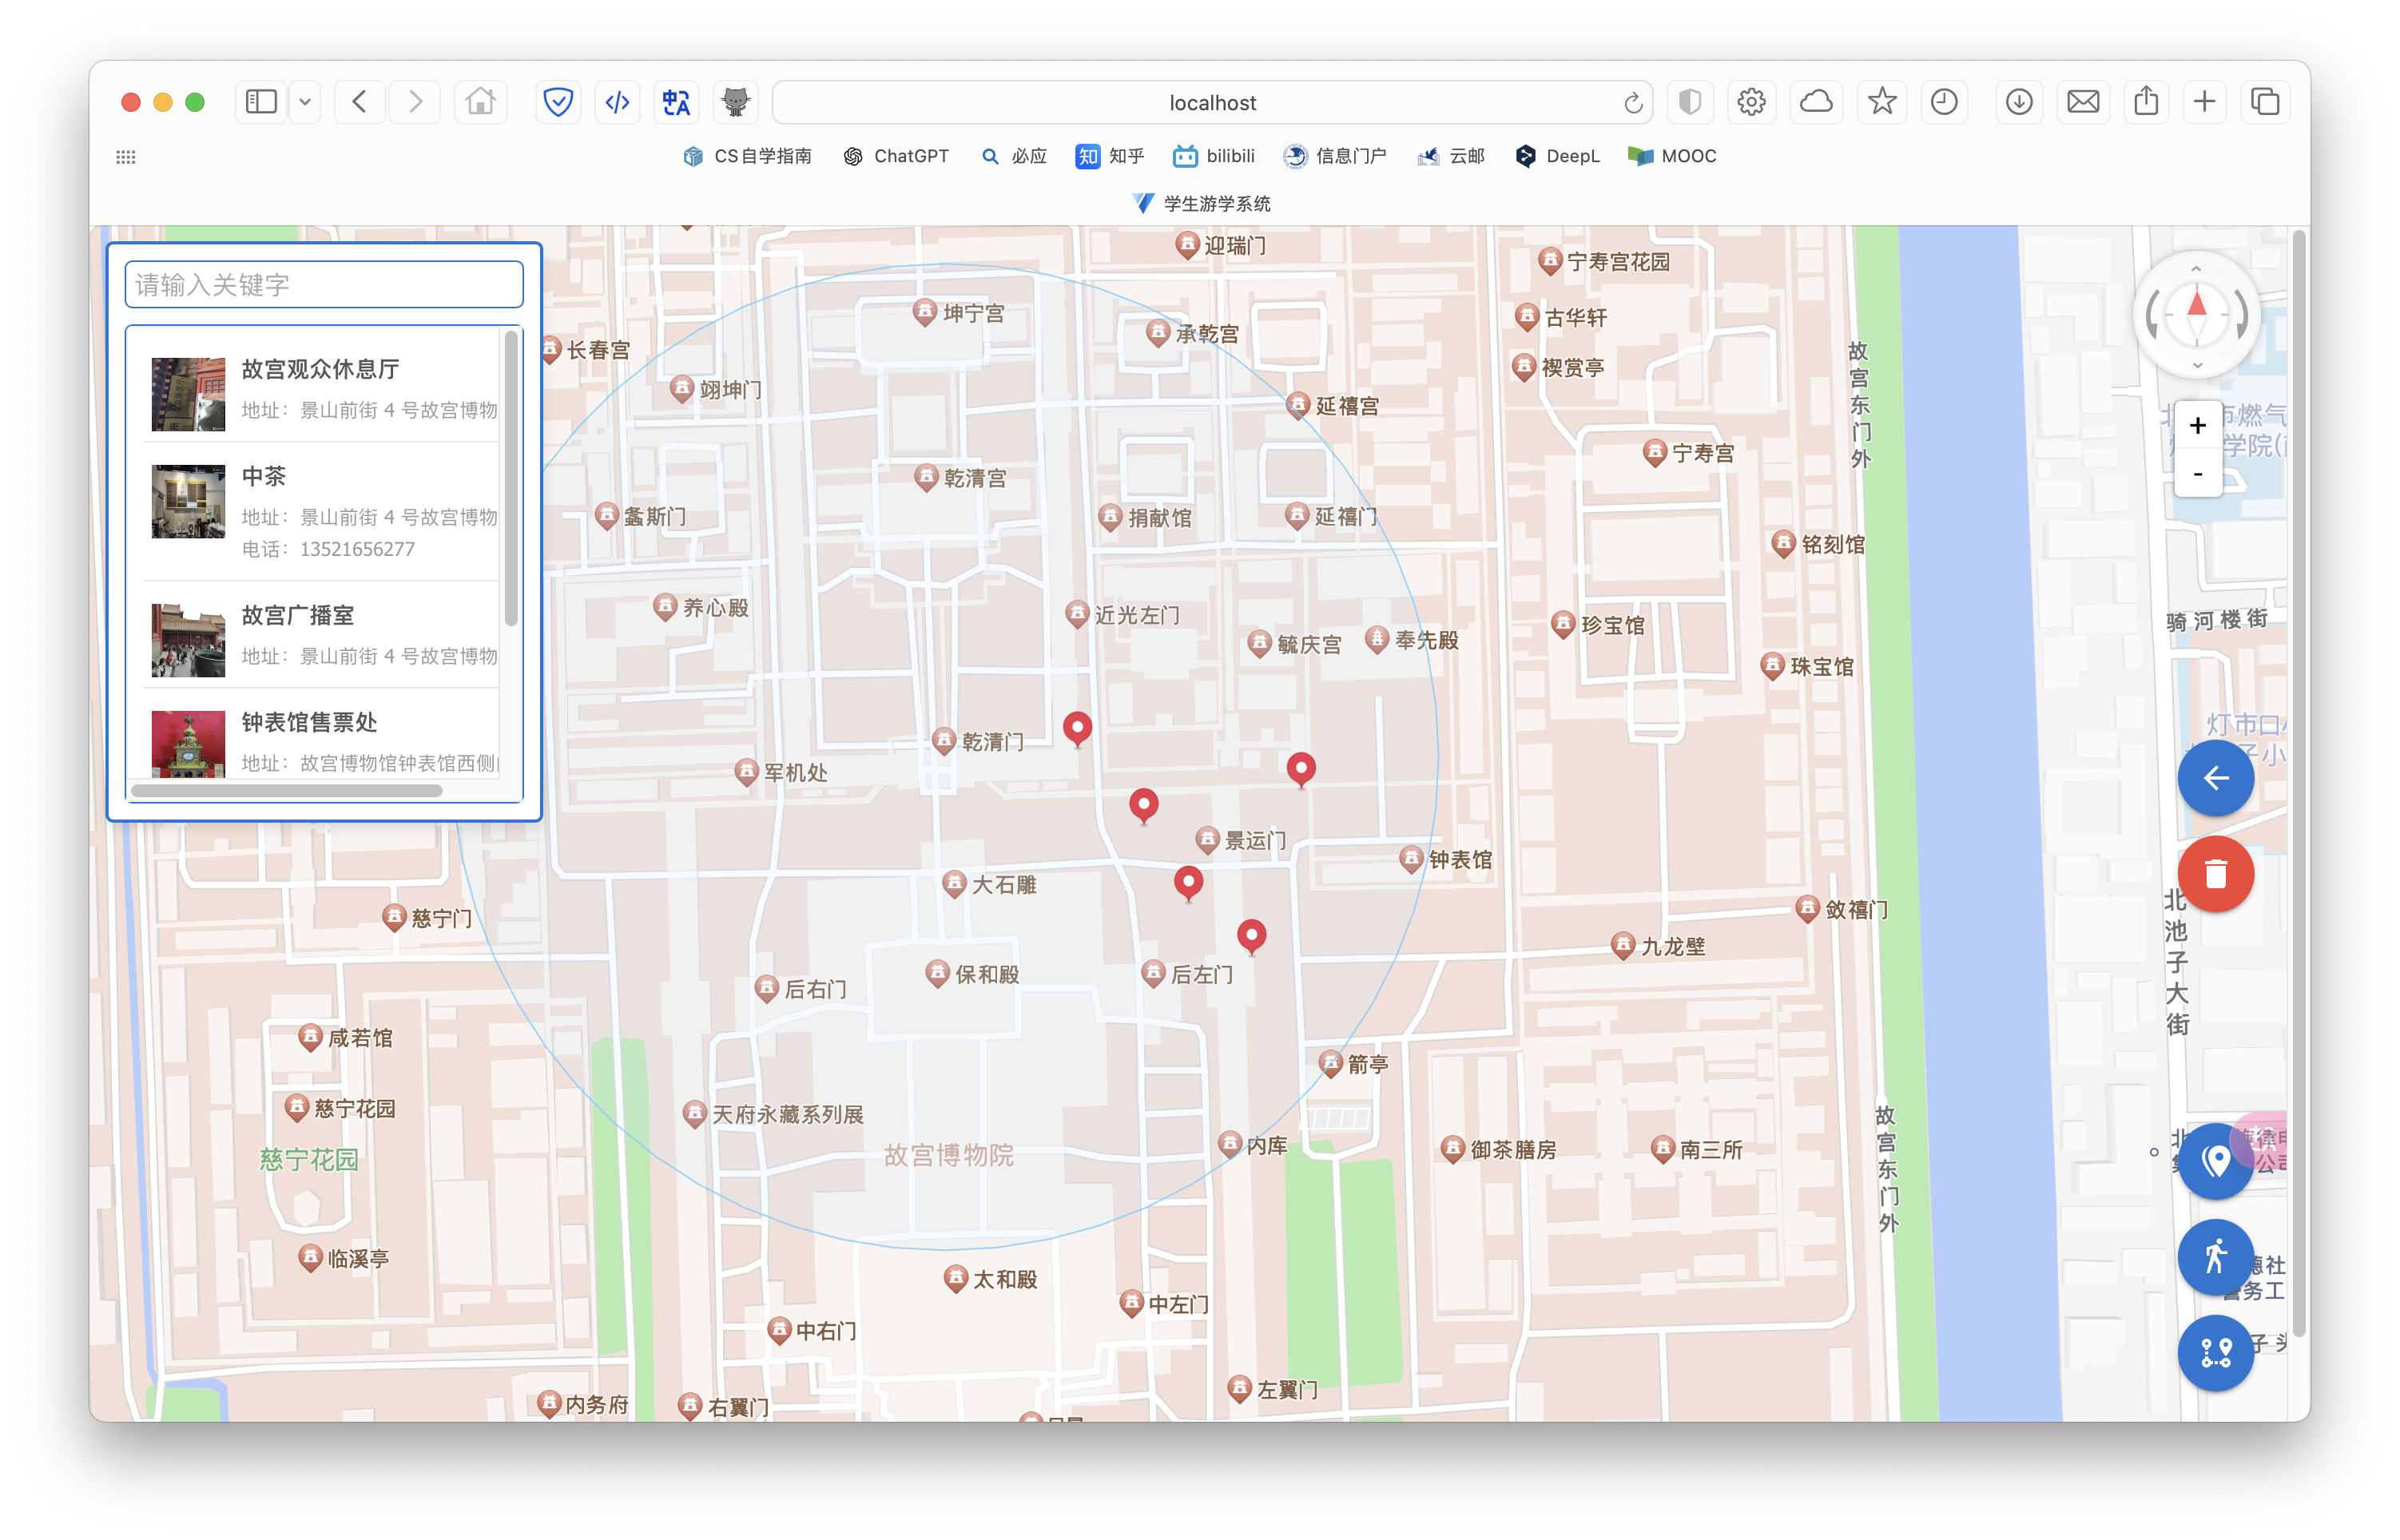
\includegraphics[width=0.85\textwidth]{figure/map.png}
    \caption{地图,周边服务及规划模式切换}
\end{figure}

\begin{figure}[htbp]
    \centering
    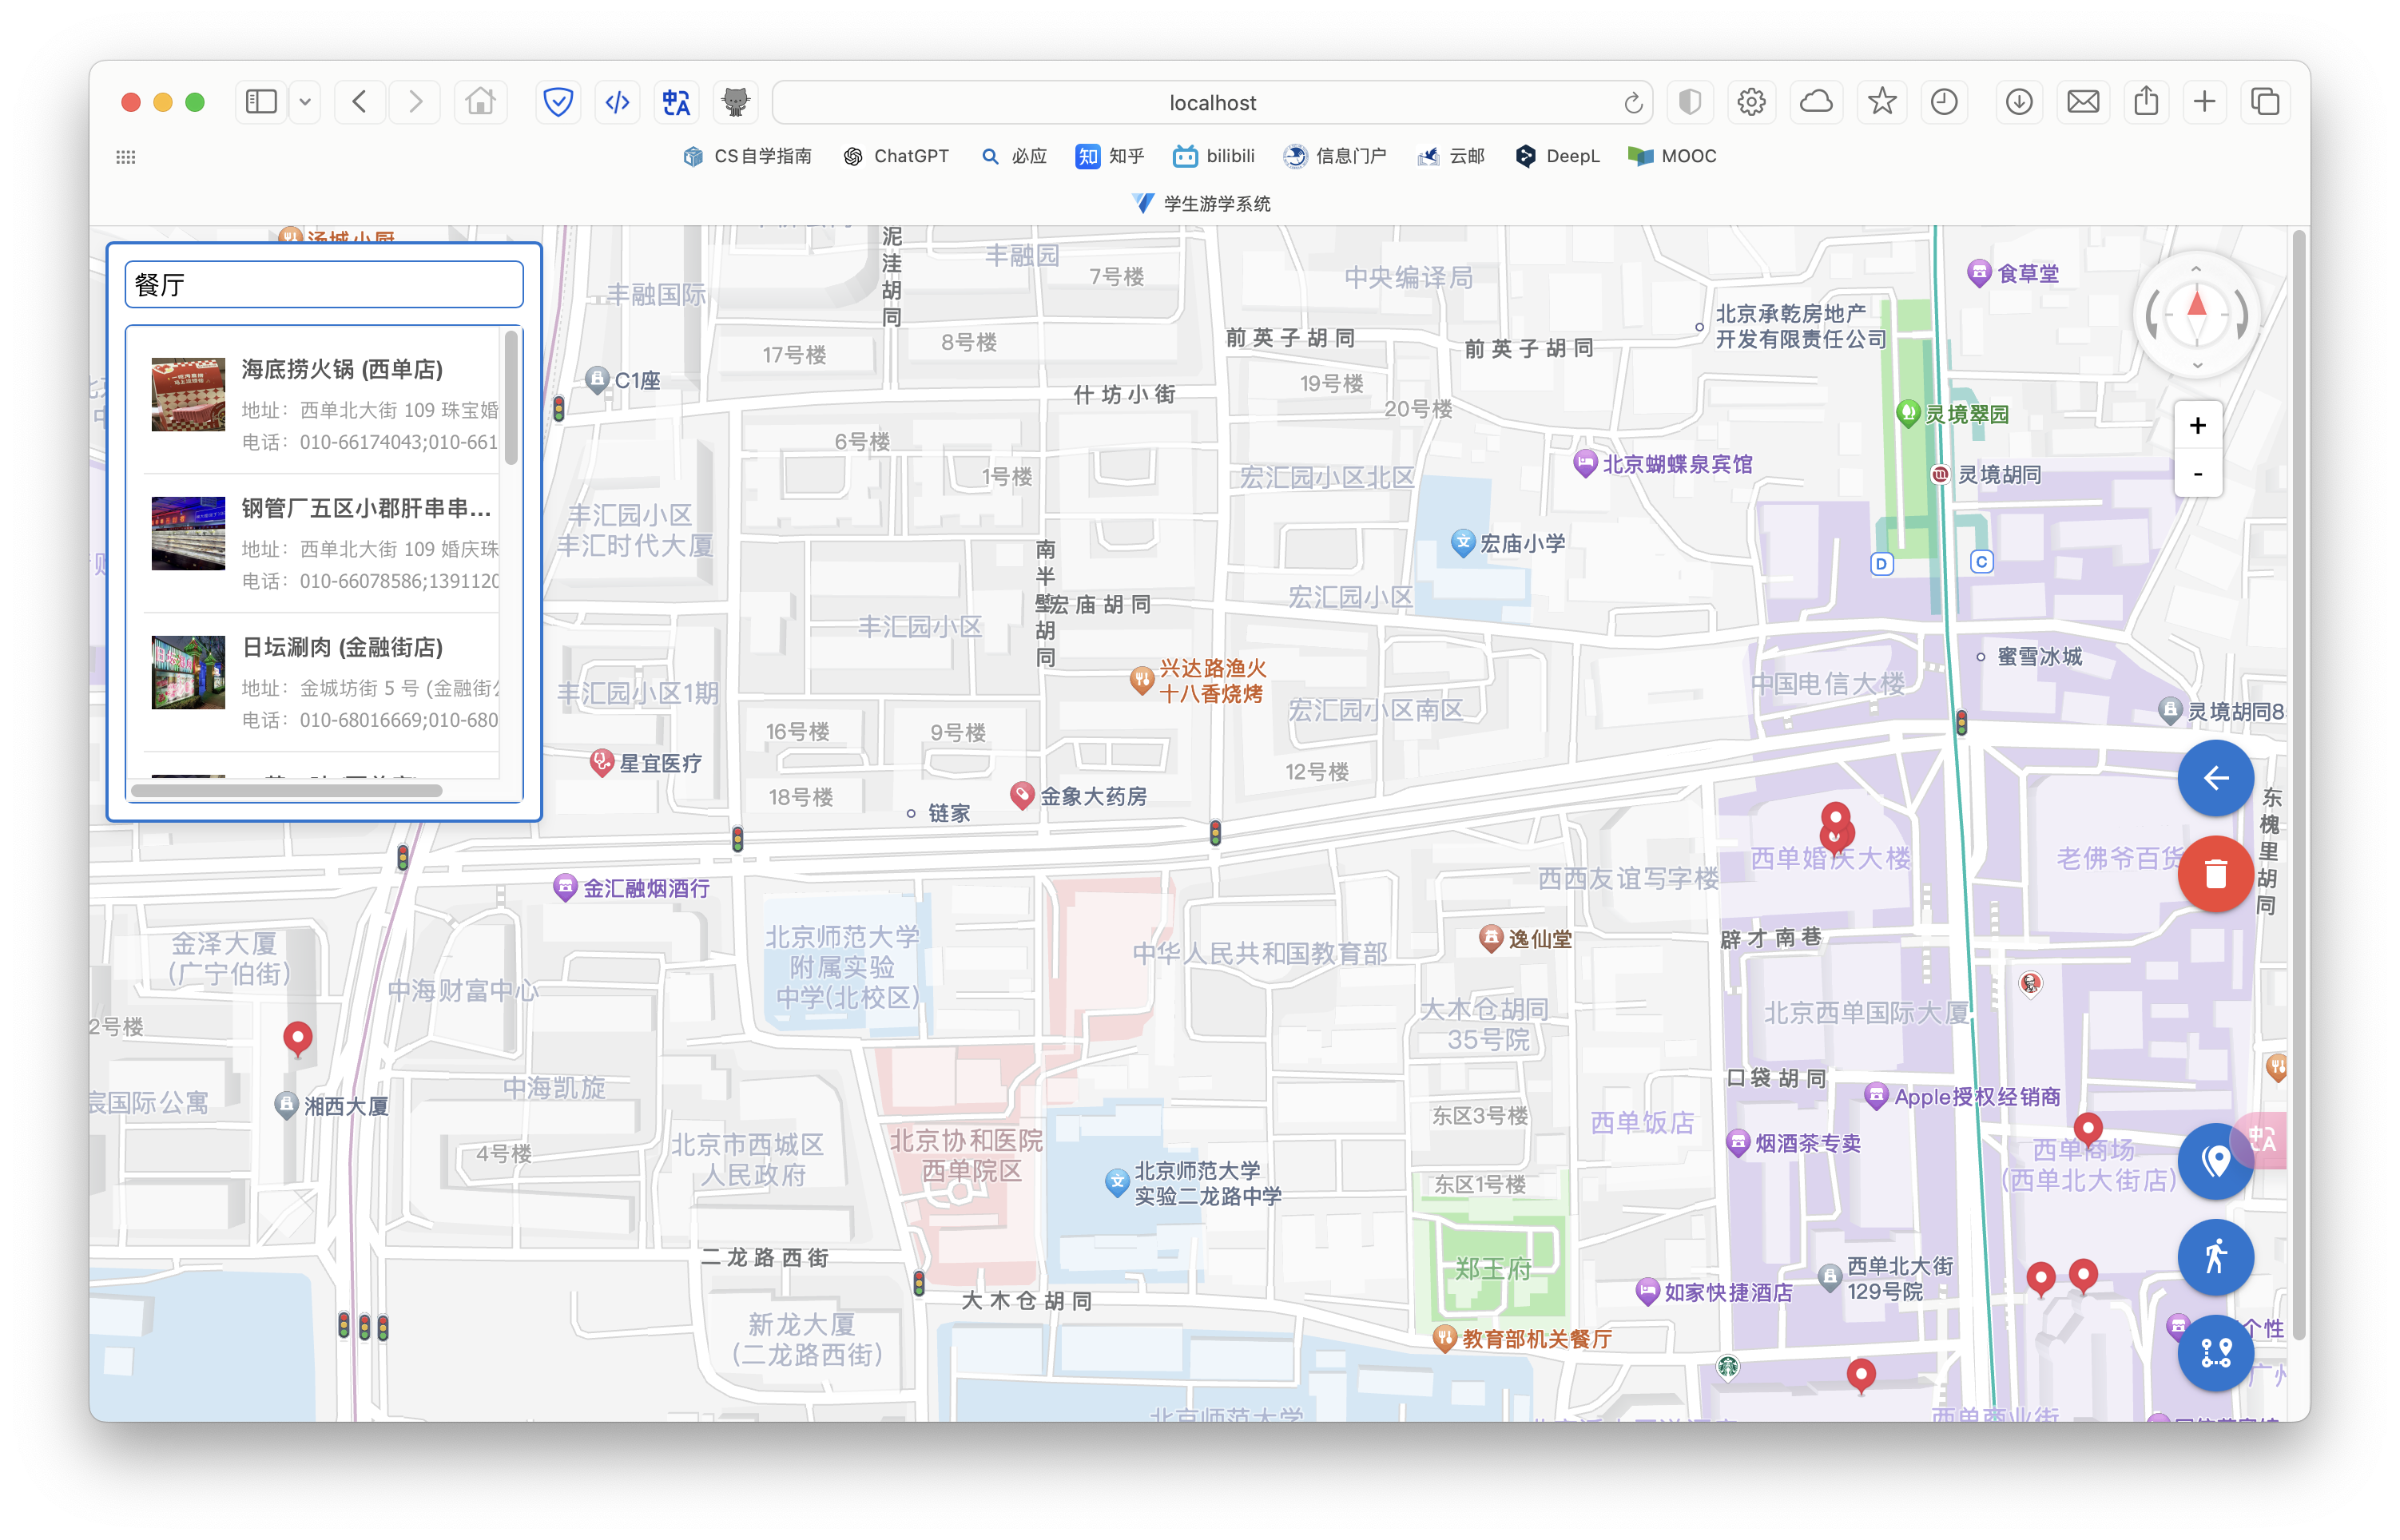
\includegraphics[width=0.85\textwidth]{figure/search.png}
    \caption{周边搜索及美食推荐}
\end{figure}

\begin{figure}[htbp]
    \centering
    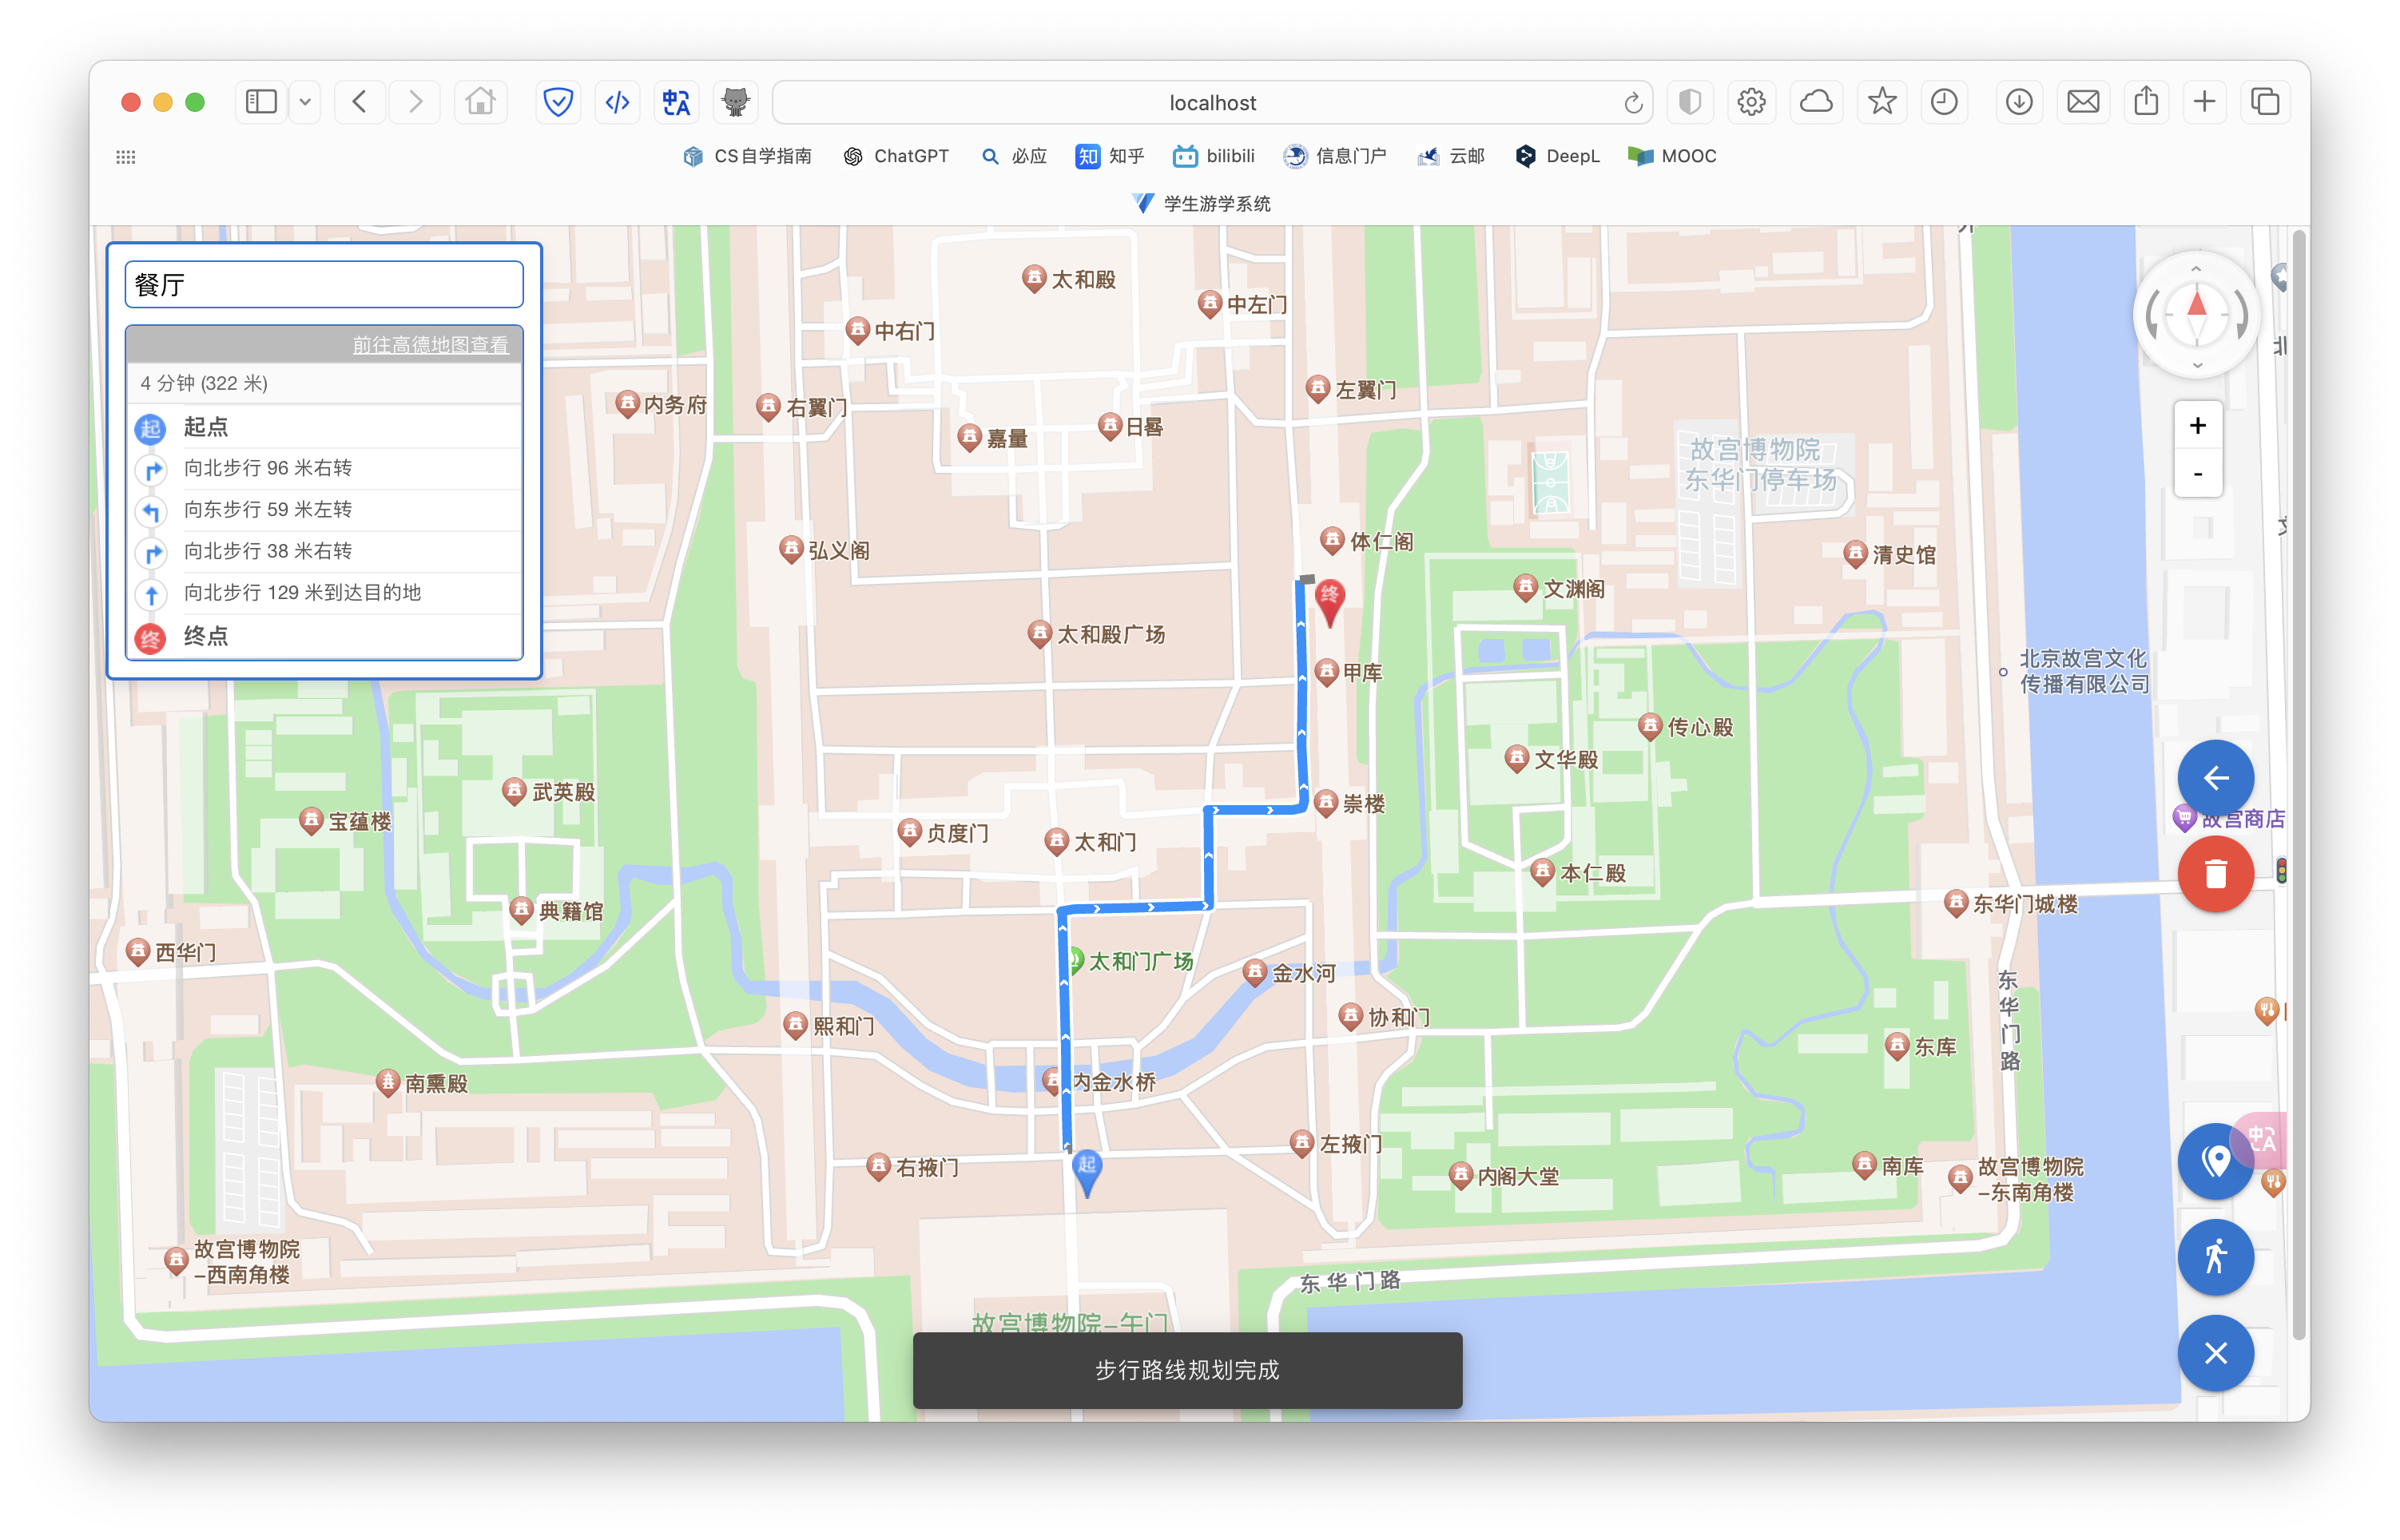
\includegraphics[width=0.85\textwidth]{figure/route.png}
    \caption{路径规划}
\end{figure}

\begin{figure}[htbp]
    \centering
    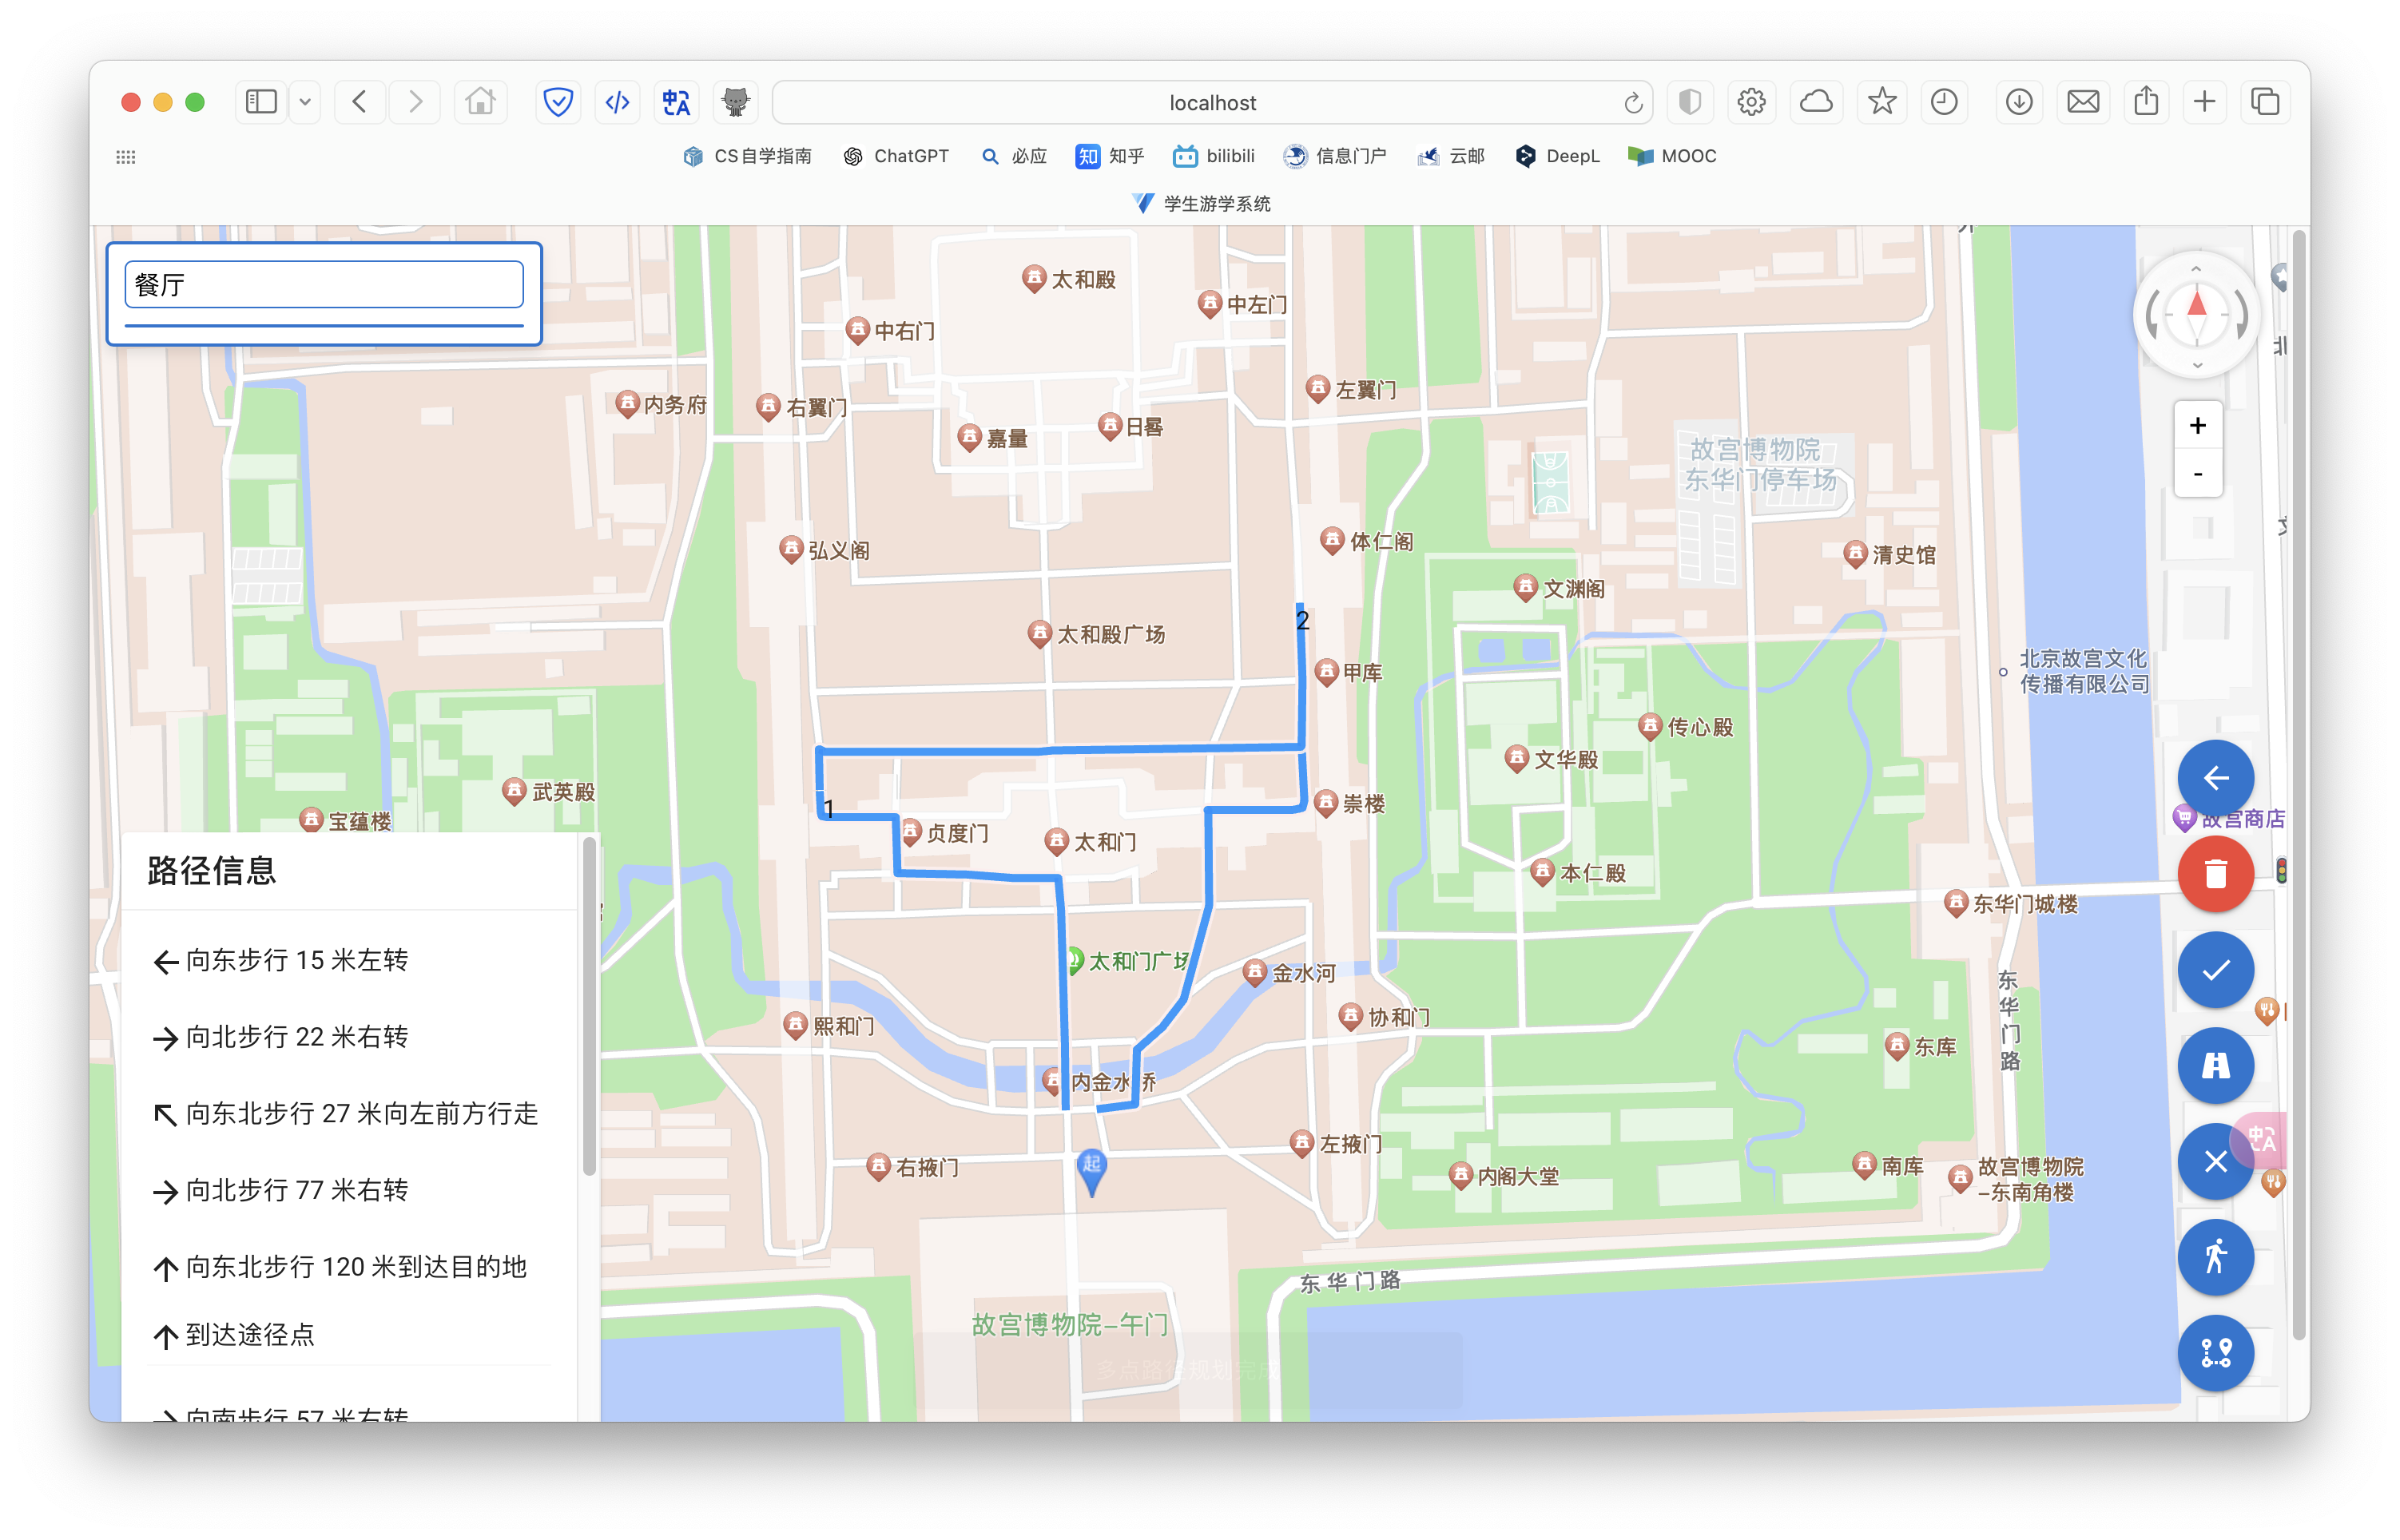
\includegraphics[width=0.85\textwidth]{figure/multi.png}
    \caption{多点路径规划及出行方式切换}
\end{figure}

\begin{figure}[htbp]
    \centering
    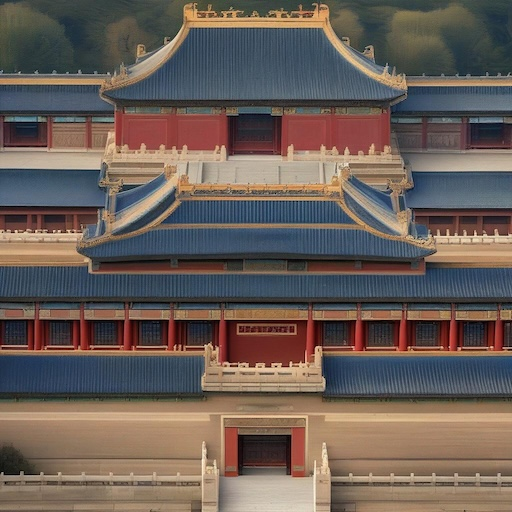
\includegraphics[width=0.8\textwidth]{figure/The_Imperial_Palace.jpeg}
    \caption{AICG生成图片}
\end{figure}

\end{document}
